\documentclass[a4paper,12pt]{article}

\usepackage[magyar, english]{babel}
\usepackage{amsmath, amssymb}
\usepackage[makeroom]{cancel}
\usepackage[utf8]{inputenc}
\usepackage{latexsym}
\usepackage{multirow}
\usepackage{datenumber}
\usepackage{graphicx}
\linespread{1.3}
\usepackage[paper=a4paper,left=20mm,right=20mm,top=10mm,bottom=15mm]{geometry}


\author{Berta Árpád}
\title{Döntéselméleti modellek gyakorlat}
\date{\today}

\begin{document}
\maketitle

Az alábbi gyakorlati jegyzet soha nem lesz készen, folyamatosan fejlődik. Amely részeket ritkábban vagy nem érintünk a gyakorlaton, azok lassabban fejlődnek, akár hibákat is tartalmazhatnak. Érdemes időnként, de leginkább számonkérés előtt felkeresni a legújabb változatát. Az anyag nagyrészt a következő könyv válogatott fejezeteire épül: 

\begin{tabular}{c}
  Temesi József: \emph{A döntéselmélet alapjai} (2002, Aula kiadó)
\end{tabular}

\tableofcontents

\

\

\

\section{Bevezetés - Többtényezős döntések}

\subsection{Egy jellemző döntési feladat - lakásvásárlási probléma}

Új városba költözéskor lakóingatlanhoz szeretnénk jutni. Ehhez feltesszük, hogy rendelkezünk egy alaptőkével, amely elegendő több lehetséges lakás (alternatívák) közül egy lakás megvásárlásához. A lakás kiválasztásához több különböző szempontot (kritériumot) kell figyelembe vennünk és ezek alapján a legjobbat kiválasztani. Ilyen például a lakás ára, mérete, beosztása, esztétikuma, külleme, a lakókörnyék közbiztonsági -, levegőminőségi szintje, kiszolgáló létesítmények (bolt, piac, kocsma, szórakozóhely), parkolási, biciklitárolási, megközelíthetőségi lehetőségek, a lakásból érzékelhető kilátás és a táj szerkezete.

\textbf{Feladat}: egyetlen cselekvési alternatíva kijelölése (pl: legjobb lakás). 

\

További példák: 
\begin{itemize}
\item politikai, üzleti, termelési döntések (közgazdaságtan)
\item ajánlórendszerek, szakértői rendszerek (adatbányászat) 
\item Temesi jegyzet 12-13 o. 
\end{itemize}

\subsection{Alapfogalmak}

\paragraph{Alternatívák:} egy döntési szituáció lehetséges megoldása, lehetséges cselekvések. Ezek strukturált halmaza: \emph{döntési tér} (v. döntési felület). Megadásuk nem feltétlenül matematikai módon történik. Példa: a szóba jöhető lakások halmaza.

\paragraph{Kritériumok:} az alternatívák azon jellemzői, amelyeket figyelembe szeretnénk venni a döntési feladatban. Ezek alapján döntünk az alternatívák közül. \emph{Metakritériumok} olyan kritérium, amely alapján a kritériumok közül tudunk választani (vagy rangsorolni).

\paragraph{Többtényezős döntési problémák:} véges (megszámlálható) sok alternatíva, véges sok kritérium. Feladat: egyetlen cselekvési alternatíva kijelölése (pl: legjobb lakás), vagy az alternatívák rangsorolása. Nincs egzakt, minden környezetben és probléma-típusra általánosan elfogadott algoritmus (ezek megismerése a félév anyaga). Nehézség: lehetnek szubjektív elemei. Teljes döntési folyamatot le kell fedni.

\paragraph{Döntéshozó:} felelős a döntés meghozásáért. Több személy is lehet (egyéni $\leftrightarrow$ csoportos döntések). Esetek többségében feltehető, hogy a döntéshozó racionális döntést hoz, optimalizáló szemléletű (Pareto-optimális alternatívák közül választ). Többek között ezt a feltevést járja körbe és cáfolja Herbert A. Simon és Daniel Kahneman (esszék) $\rightarrow$ \emph{korlátozott racionalitás}: kielégítő szemlélet (ez inkább az általános). Döntéshozó az objektív adatok ismeretén felül \emph{preferenciákkal} rendelkezik, ezek alapján dönt.

\section{Bevezetés - Lineáris programozás}

\paragraph{Többcélú programozási feladat: }

Fontos kiemelni, hogy amennyiben a feladatunk feltétel-rendszer és célok különválasztásából és egy matematikai programozási modell feladat felírásából tevődik össze, akkor hagyományos módon többcélú programozási feladatról beszélünk (feladat típusától függően akár LP, vagy hozzárendelési feladat, vagy szállítási feladat). A változók folytonos és egész értékűek és a hozzájuk megadott korlátokkal       testesítik meg a döntési szempontrendszerünk. Ilyen esetben a legjobb döntés kiválasztását célfüggvény vezérli és matematikai feladatként megoldható \textbf{(így nem a többtényezős döntési problémákra ismertetett eljárásokkal foglalkozunk ilyen esetben)}.

\textbf{Probléma}:
\begin{itemize}
\item több alternatív (akár szélsőségesen eltérő struktúrájú) optimum lehet és ezek (alternatívák) közül választani kell $\rightarrow$ valamilyen pótlólagos információra van szükség.
\item az esetek döntő többségében nehéz (sőt lehetetlen) a döntési problémát egyetlen célfüggvény kiértékelésére leegyszerűsíteni.
\end{itemize}
  
\paragraph{ Egy példa feladat: } Többféle termék előállításának mennyiségéről kell döntenünk. Döntésünket elsősorban a korlátozottan rendelkezésünkre álló erőforrások (nyersanyag-, munkaerő- és költségkorlátok), illetve a termelés technológiai szabványai befolyásolják. Az elérendő cél a maximális profit, minimális környezeti kár okozásával, illetve lehető legnagyobb társadalmi fejlődés elérésével.

\paragraph{ Optimum-fogalom: } Amennyiben több célfüggvény is van $\rightarrow$ új optimum-fogalom kell. \emph{Pareto-optimum} több cél egyidejű teljesülése úgy, hogy nem lehet olyan újabb lehetséges megoldást megadni, ami minden szempontból nem rosszabb az előzőnél, és egy szempont szerint jobb az előzőnél. Ezeknek a halmaza viszont általában végtelen sok elemből áll  $\rightarrow$ nem alkalmas a döntési probléma megoldására. Kompromisszumos megoldást kell keresni. Lehetőségek (mindegyik egyetlen cfgv-re vezeti vissza a megoldást):

\begin{itemize}
\item súlyozásos módszer: célfüggvényekhez fontossági súlyokat rendelünk, súlyokkal képzett összegként áll elő az egyetlen cfgv (nehéz a súly megadása)  
\item lexikografikus módszer: legfontosabb cfgv lesz a cfgv (melyik a legfontosabb?)
\item korlátok módszere: egy cfgv-t kiválasztunk a többit beépítjük a feltételrendszerbe (mi lesz a korlát?)
\item kompromisszumprogramozás elve: kiszámoljuk minden cfgv szerinti legjobb értéket és azt az alternatívát (megoldást) választjuk, ami ehhez a legközelebb van (mi a távolságfüggvény?)
\end{itemize}


\section{Bevezetés - Döntési folyamat:}

\begin{enumerate}

\item döntési helyzet keletkezése $\rightarrow$ konfliktus (fel kell oldani, dönteni kell)
\item döntési probléma megfogalmazása és formalizálása
	\begin{enumerate}
	\item a döntési cél megfogalmazása
	\item alternatívák kijelölése
	\item kritériumok meghatározása
	\end{enumerate}
\item módszer választás (nehéz)
\item megoldás: egyetlen cselekvési lehetőség kiválasztása (vagy alternatívák egyértelmű rangsorolása)
\item kiértékelés, elemzés (helyes volt-e a döntésünk?)
\end{enumerate}

\section{Bevezetés - Döntéstámogató rendszerek (DSS):} Célja a döntési folyamat automatizálása, döntési feladat megoldásának a segítése. Hagyományosan célorientált (domain specifikus) rendszerek.

Megkülönböztetünk:
\begin{itemize}
\item Passzív DSS: felügyeli a döntési folyamatot, de nem ajánl fel semmilyen döntési lehetőséget (kritikai rendszerek)
\item Aktív DSS: felügyeli a döntési folyamatot, konkrét javaslatot ad a döntésre
\item Kooperatív DSS: a döntési folyamat közben is lehetőség van az egyes paraméterek módosítására, az eljárás újradefiniálásra
\end{itemize}

\paragraph{Eszközök: } egyes folyamatok automatizálása, vizualizáció, szűrés -, súlyozás -, preferencia -, hasznosság alapú módszerek (minden a félév során megismert eljárás), ajánlórendszerek, gépi tanulás, adatbányászat, szövegbányászat, tudásalapú -, szakértői rendszerek, többcélú programozás, megerősítéses tanulás, ... 

\section{Bevezetés - Csoportos döntések:}

Akkor beszélünk csoportos döntésről, ha a döntés nem egyetlen döntéshozótól függ, hanem több döntéshozó van $\longrightarrow$ elosztott döntés.

\begin{itemize}
\item vertikális: a folyamat egyes részeit osztjuk szét különböző döntéshozókhoz, mindenki az adott részfeladatban \emph{egyedül} dönt. A döntések közötti kapcsolatot kell megadnunk, a részdöntésekre pedig a hagyományos DSS-eket alkalmazhatjuk.

\item horizontális: egy döntési kérdésben több döntéshozó dönt $\longrightarrow$ szavazási eljárások. DSS vezérli a szavazást, vagy egy aktív DSS is lehet egy döntéshozó. 
\end{itemize}

\paragraph{Szavazási eljárások}

A szavazás során egy olyan \emph{társadalmi jóléti függvény}t keresünk, amely méltányosan összegzi az alternatívák feletti preferenciákat $\longrightarrow$ helyes rendezést ad az alternatívákra. Helyes rendezés alatt olyan csoportos döntést értünk, ami az alábbi tulajdonságokat egyidejűleg kielégíti:

\paragraph{Megkövetelt tulajdonságok: }
\begin{itemize}
\item Univerzális értelmezési tartomány: minden lehetséges bemenetre tud rendezést adni.

\item Gyenge Pareto elv: ha valamely alternatívát minden döntéshozó egyértelműen jobban preferál egy másiknál, akkor az a végső döntésben is jobban fog szerepelni.

\item Bináris függetlenség: felteszi, hogy minden alternatíva pár esetében csak és kizárólag az a két alternatíva befolyásolja a döntéshozókat a preferenciarendezésben.

\item Diktátor mentesség: nincs olyan döntéshozó, akinek a döntése dominálja az összes többiét.

\paragraph{Arrow-tétel:}
Nem létezik olyan társadalmi jóléti függvény amelyben ez a négy feltétel egyidejűleg teljesülne. $\longrightarrow$ nincs egy tökéletes szavazási eljárás.

\end{itemize}



\section{Eliminációs módszerek}

Formalizáljuk a lakásvásárlási példánkat. Tegyük fel, hogy hosszas gondolkodás után sikerült kritériumaink közül elhagyni azokat, amelyek kevésbé fontos szempontok, így végül a vizsgálataink során az alábbi jellemzők maradnak: 

\begin{itemize}
\item $X_{1}$: ára (millió forint) (kritérium: minél olcsóbb)
\item $X_{2}$: mérete (m$^{2}$) (kritérium: $70m^2$-hez közeli)
\item $X_{3}$: esztétikuma (kritérium: minél jobb)
\item $X_{4}$: környék jósága (kritérium: minél jobb)
\item $X_{5}$: bicikli tárolási lehetőség (kritérium: minél jobb)

\end{itemize}

A fenti szempontok szerint nekiálltunk lakást keresni és végül a következő négy lehetséges lakásjelöltre tudtuk redukálni a döntési terünket:
\begin{center}
\begin{tabular}{c||c|c|c|c|c}
 & $X_1$& $X_2$& $X_3$& $X_4$& $X_5$ \\
 \hline
 $A_1$&25  &98 & lepukkant & közepes & lakáson belül \\
 $A_2$&50  &56 & új& kiemelkedően jó& fedett \\
 $A_3$&45  &120 & újszerű & kifejezetten rossz& nyitott udvaron \\
 $A_4$&52  &56 & új& kiemelkedően jó& fedett \\
\end{tabular}
\end{center}

\subsection{Dominancia módszer}

\paragraph{Dominált alternatíva:} olyan alternatíva, ami egyik kritérium szerint sem jobb, és legalább egy szempont szerint rosszabb egy másik alternatívánál.  A nem dominált alternatívák egyben Pareto-optimális megoldások.

A módszer lényege ezek kiszűrése (eliminációs módszer). Amennyiben dominált alternatívát választana egy döntéshozó, akkor az nem számítana racionális döntésnek. 

A példában az $A_4$ egy dominált alternatíva: egyik szempont szerint sem jobb az $A_2$-nél, és az $X_1$ kritérium szerint rosszabb. 

\subsection{Kielégítésre törekvő módszer}

Minden célhoz meghatározunk egy \emph{kielégítési szintet}. Ez lényegében azt jelenti, hogy mi az a szint (\textbf{szükségességi feltétel}), az adott szempontból, ami felett (v. alatt) elfogadnánk az adott alternatívát. Például: közepes közbiztonsági szint felett már elgondolkozunk a lakás megvásárlásán. Ezek alapján kiküszöbölhetőek azok az alternatívák, amik valamilyen szempontból már nem elfogadhatóak a számunkra. Azok az alternatívák maradnak, amelyek minden kielégítési szintnek megfelelnek. Tehát minden szempontból megbízható. Ugyanakkor általában nem feltétlenül ilyet keresünk, sőt a legjobb alternatívát is kiszórhatja, ami egyébként éppen a határérték alatt van egy szempont szerint. A módszer alkalmazásakor nem az egyetlen legjobb alternatívát keressük, hanem megpróbáljuk szűkíteni az alternatívák halmazát (eliminációs módszer). 

\subsection{Diszjunkt módszer}

Az előző módszer kifordítva. Nem egy minden szempontból megbízható alternatívát keresünk, hanem olyat ami valamilyen (akár több) szempontból kiemelkedő. Módszer: minden szemponthoz meghatározzuk azt a szintet (\textbf{elegendőségi feltétel}), amelynél ha egy alternatíva jobb értékkel bír, akkor bent marad az alternatívák halmazában. Ha egy szempont szerint sem kiemelkedő, akkor elvetjük. Ebben az esetben is szűkítjük az alternatívák halmazát és nem egyetlen legjobbat keresünk (eliminációs módszer).

Példa: 30 millió forint alatti ingatlanokat kiemelkedően jó értékűnek tartjuk. A 70 m$^2$-hez képest legfeljebb 15 m$^2$-rel eltérő ingatlanokat kiemelkedően jó alapterületűnek tartjuk. ...


\section{Elemi döntési módszerek (determinisztikus modellekre)}

\paragraph{Problémák az eddigi ábrázolással:}
\begin{itemize}
\item nem számszerű értékek,
\item normalizálatlan (nem ismert a globális range),
\item kritériumonként eltérően maximalizálni vagy minimalizálni szeretnénk, 
\item a lakás mérete esetében pedig általában inkább egy megfelelő értéket szoktunk keresni és nem minél nagyobb vagy minél kisebb méretű lakást (tegyük fel, hogy \textbf{70 m$^2$}-es a számunkra optimális lakásméret).
\end{itemize}
\paragraph{Szubjektív értékelések számszerűsítése:}

Ezt majd részletesen fogjuk vizsgálni az értékelő- függvények tárgyalásakor. Most bemondásos alapon határozzuk meg az értékeket:

\begin{center}
\begin{tabular}{cccc}
lepukkant& felújításra szorul& újszerű & új \\
0.2 &0.3&0.6&0.9\\
\end{tabular}

\begin{tabular}{ccc}
 kifejezetten rossz& közepes & kifejezetten jó \\
 0.12&0.56&0.97\\
\end{tabular}

\begin{tabular}{cccc}
 nincs & lakáson belül & nyitott udvaron & fedett \\
 0.0 & 0.1 & 0.5 & 0.9 \\
\end{tabular}

\end{center}

A lakás méretének egyirányú skálára való felfűzése több lehetséges módon is történhet. A legegyszerűbb ha a keresett optimális értéktől vett euklideszi távolságot vesszük. Ha nagyobb irányba térünk el, akkor az a túlzott fűtési költségek miatt kedvezőtlen, ha pedig kisebb méret irányába, akkor pedig a kevés hely miatt kedvezőtlen. Ebben az esetben feltesszük, hogy mind a két irány azonos súllyal ront a lakás "jóságán".

\begin{center}
\begin{tabular}{c||c|c|c|c|c}
 & $X_1$& $X_2$& $X_3$& $X_4$& $X_5$ \\
 \hline
 $A_1$&25  &28 & 0.3 & 0.56 & 0.1 \\
 $A_2$&50  &14 & 0.9 & 0.97& 0.9 \\
 $A_3$&45  &50 & 0.6 & 0.12& 0.5 \\
 $A_4$&52  &14 & 0.9 & 0.97& 0.9 \\

\end{tabular}
\end{center}

\paragraph{Skála meghatározása:} szakértőktől, vagy ha nem jutunk semmilyen információhoz, akkor az ismert értékek maximuma és minimuma alapján.

\paragraph{Normalizálás:} 
\begin{center}
maximum feladat: $r_{ij} = \frac{x_{ij} - x^{min}_j}{x^{max}_j - x^{min}_j} $ 

minimum feladat: $r_{ij} = \frac{x^{max}_j - x_{ij}}{x^{max}_j - x^{min}_j} $
\end{center}
Maximum és minimum meghatározása:
\vspace{-0.2cm}
\begin{itemize}
\item az ismert értékekből kijelölve
\vspace{-0.3cm}
\item szakértői segítséggel
\end{itemize}

\begin{center}
\begin{tabular}{c||c|c|c|c|c}
 & $X_1$& $X_2$& $X_3$& $X_4$& $X_5$ \\
  &\small{$max=100,$}&\small{$max=70,$}	&		&		&	\\
 &\small{$min=10$}&\small{$min=0$}	&		&		& \\
 \hline
 $A_1$&0.83  &0.6 &  0.3 & 0.56 & 0.1 \\
 $A_2$&0.56  &0.8 & 0.9 & 0.97 & 0.9 \\
 $A_3$&0.61  &0.29 & 0.6 & 0.12 & 0.5 \\
 $A_4$&0.53  &0.8 & 0.9 & 0.97 & 0.9 \\
\end{tabular}
\end{center}

\subsection{Lexikografikus módszer}

A célok között fontossági sorrendet állítunk fel. Ezután választjuk a legfontosabb szempontot, megnézzük, hogy eldönti-e az alternatívák választását. Ha egy kiemelkedik akkor azt választjuk, ha nem akkor folytatjuk a második legfontosabb döntéssel mindaddig, míg egyetlen alternatíva nem marad.

Pl: legfontosabb szempont, hogy a biciklitárolási lehetőség, második pedig a lakás ára. Ebben az esetben a legfontosabb cél szerint két alternatíva marad, de a lakás ára alapján már egyértelműen lehet dönteni a fennmaradó két alternatíva közül.

\subsection{Maximin módszer (pesszimista döntéshozó)}

Az értékek azonos, normalizált skálán vannak. Minden alternatívához megkeresi a felvett leggyengébb értéket és azok közül kiválasztja a legjobbat.

A példában az utolsó alternatíva legrosszabb értéke 0.53, az $A1$-é 0.1, az $A2$-é 0.56, míg az $A3$-é 0.12, így ezeknek a maximuma 0.56, ezért az $A2$ alternatívát választjuk.

\subsection{Maximax módszer (optimista döntéshozó)}

Minden alternatívához megkeresi a felvett legjobb értéket és ezek közül kiválasztja a legjobbat.

A példában az $A1$ alternatíva maximális értéke 0.83, az $A2$-é és az  $A_4$-é  0.97, míg az $A3$-é 0.61. Mivel több alternatíva maradt ezért közülük az eddigi kritériumok letakarásával a következő maximális érték mentén próbálunk dönteni, mindaddig, míg nem lesz egyértelmű legjobb alternatíva. Az ár szerint már egyértelmű döntést tudunk hozni: $A_2$.


\subsection{Súlyozásos módszer}

Minden kritériumhoz meghatározunk egy súlyt és elvárjuk, hogy a súlyok összege 1 legyen. Majd a súlyozott összegek alapján a maximális értékű alternatívát választjuk. 

Például legyen a döntéshozó akarata alapján az $X_1$-hez tartozó súly 0.5, míg az $X_2$, $X_3$, $X_4$-hez 0.1, illetve az $X_5$-höz 0.2. A súlyok összege 1, tehát megfelelő súlyozást adott meg a döntéshozó. Ezek alapján kiszámoljuk az egyes alternatívákhoz kapcsolódó súlyozott összegeket. Az $A_1$ alternatíva esetében $0.5\cdot0.83+0.1\cdot0.6+0.1\cdot0.3+0.1\cdot0.56+0.2\cdot0.1$, ami 0.581. Az $A_2$ esetében ugyanez 0.727, az $A_3$ esetében 0.506, míg $A_4$ esetében 0.712. Mivel a maximális értéket az $A_2$ veszi fel, ezért ezt az alternatívát választjuk. 


\

A skálák meghatározásának nehézségére és az egyes kritériumok értékeinek becslésére megoldás: értékelő függvény alkalmazása.

\section{Értékelő függvények}

%Ilyen függvényeket a determinisztikus döntési modell esetében vizsgálhatunk. Amennyiben sztochasztikus modellünk van akkor az \ref{sec:utility}. fejezetben bemutatott hasznosságfüggvényt lehet használni.

\paragraph{Preferencia reláció: } Adott értékelésre váró alternatívák $A$ halmaza (akár véges vagy végtelen számosságú). Ebből vegyünk egy $(a,b)$ rendezett elempárt és definiáljunk felettük egy "legalább olyan jó, mint" relációt ($\succeq$). Tehát $a \succeq b$ akkor és csak akkor, ha $a$ legalább olyan jó mint $b$. 

\small{(Nagyon sok más preferencia alapú döntési módszer létezik, ezekből egy az értékelő függvény alapú)}

\paragraph{Értékelő függvény: }  $v: A \rightarrow \mathbb{R}$ , ahol $v(a) \geq v(b) \Leftrightarrow a \succeq b$

\subsection{Preferenciareláció tulajdonságai}

\paragraph{További relációk bevezetése:}

\begin{itemize}
\item \textbf{indifferencia:}  teljesül $a \succeq b $ és $b \succeq a$ is $\Rightarrow a \sim b$
\item \textbf{nem összehasonlíthatóság:}  nem teljesül se a $a \succeq b $ és se a $b \succeq a $  $\Rightarrow a$ ? $b$
\item \textbf{szigorú preferencia:} teljesül $a \succeq b $, de $b \succeq a$ nem teljesül $\Rightarrow a \succ b$ ($a$ egyértelműen jobb, mint $b$)
\end{itemize}

\paragraph{Definícióból adódó fontos tulajdonságaik:}

\begin{itemize}
\item \textbf{preferencia reláció reflexív: } $a \succeq a $, tehát $a$ legalább olyan jó, mint $a$ mindenképpen teljesül 
\item \textbf{indifferencia reflexív:} $a \sim a $, $a$ mindenképpen indifferens $a$-hez.
\item \textbf{indifferencia szimmetrikus:}  $b \sim a \Rightarrow a \sim b$  
\end{itemize}

Ahhoz, hogy $v$-t megkonstruáljuk a $\succeq$-nak gyenge rendezésnek kell lennie. $\textbf{Gyenge rendezés: }$  reflexív, tranzitív és teljes. \textbf{Kikötjük, hogy $\succeq$ legyen gyenge rendezés.}
\begin{itemize}
\item A reflexivitás a definíció alapján teljesül. 
\item Emellé felvesszük, hogy \textbf{$\succeq$ tranzitív}, tehát \textbf{$a \succeq b$ és $b \succeq c$} estén teljesülnie kell \textbf{$a \succeq c$} (ez nehéz!! foci \textbf{körbeverés} példa, racionális döntéshozó). 
\item A teljességhez teljesülnie kell, hogy $\forall (a,b) \in A: a \succeq b$ vagy $b \succeq a$. \textbf{Nem adhatunk "nemtudom" választ, nincs ?, minden elemre meg kell adni a preferenciát}.  
\end{itemize}
Következmények:  $\sim$ is tranzitív lesz. Tehát a \textbf{$\sim$ ekvivalencia reláció} (reflexív, tranzitív, szimmetrikus). Ennek köszönhetően $\sim$ \textbf{indifferencia osztály}okat generál $A$ felett (azok az alternatívák, amik ugyanolyan jók, azonos indifferencia osztályba sorolhatók).

Az \textbf{indifferencia osztályok halmaza megszámlálható}: ez azt jelenti, hogy az alternatívák véges sok osztályba sorolhatóak. Ennek a következménye, hogy a természetes számokat felhasználhatjuk az osztályok jelölésére.

Felmerül a kérdés, hogy milyen az, ha az indifferencia osztályok halmaza nem megszámlálható? Például, amennyiben tökéletesen osztható javak tartoznak az infifferencia osztályokba, melyeknek tovább osztásával újabb osztályok hozhatóak létre.

Minden adott $v$ létezéséhez.

\subsection{Értékelő függvény létezése}

Ha a $\succeq$ reláció gyenge rendezés az $A$ halmaz elemeire vonatkozóan, és az indifferencia osztályok halmaza megszámlálható $\Rightarrow \exists v: A \rightarrow \mathbb{R} $, ahol $\forall(a,b) \in A$ teljesül, hogy 
\begin{itemize}
\item $a \succeq b \Leftrightarrow$  $v(a) \geq v(b)$, (vagy
\item $a \succ b \Leftrightarrow v(a) > v(b)$, és $a \sim  b \Leftrightarrow v(a) = v(b).$)
\end{itemize}
(Bizonyítás Fishburn (1970), de nem kell itt, mert nem konstruktív)



\paragraph{Tulajdonságok:}

\begin{enumerate}

\item A $v$ értéke általában a [0,1] intervallumra skálázódik és a 0 jelenti a legrosszabb preferencia értéket és az 1 a legjobbat. Közbeeső értékek megegyeznek a preferenciarendezés értékeivel.

\item Számszerű értéket ad arra, hogy egyik alternatívát jobban preferáljuk a másiknál. Növekvő preferencia sorrend $\rightarrow$ az értékelő függvény \textbf{monoton növekvő} (ez eltérhet, de azt nem vizsgáljuk).

\item \textbf{Stratégiailag ekvivalens} értékelő függvények: az alternatívákhoz ugyan azt a preferencia sorrendet határozza meg.


\item Racionális a döntéshozó $\Rightarrow$ létezik értékelő függvény.

\end{enumerate}

%\begin{center}
%\begin{tabular}{c||c|c|c|c|c}
% $A$ & $X_1$& $X_2$& $X_3$& $X_4$& $X_5$ \\
% \hline
% $a_1$&$v_1(x_{a_1,1})$  &$v_1(x_{a_1,2})$ & $v_1(x_{a_1,3})$ & $v_1(x_{a_1,4})$& $v_1(x^1_{5})$ \\
% $a_2$&$v_1(x_{a_2,1})$  &$v_1(x_{a_2,2})$ & $v_1(x_{a_2,3})$ & $v_1(x_{a_2,4})$& $v_1(x^2_{5})$ \\
% $a_3$&$v_1(x_{a_3,1})$  &$v_1(x_{a_3,2})$ & $v_1(x_{a_3,3})$ & $v_1(x_{a_3,4})$& $v_1(x^3_{5})$ \\
%\end{tabular}
%\end{center}

\paragraph{A fenti tétel, túl szigorú az indifferencia osztályok megszámlálhatóságáról.}

Ha gyengítjük a feltételt akkor is megkaphatjuk $v$ létezését.

Legyen a feltételünk az, hogy $\exists B$ az indifferencia osztályok egy részhalmaza, amelyre teljesül:
\begin{itemize}
\item $B$ megszámlálható,
\item $\forall A_1, A_2$ indifferencia osztály részhalmazra: $\exists C \in B$, hogy ha $A_1 \succ A_2$ akkor $A_1 \succ C \succ A_2$ (tehát sűrű a $\succ$ rendezésre). 
\end{itemize}
Ekkor teljesül $v$ létezése. Összefoglalva ez annyit jelent, hogy ha létezik olyan véges indifferencia osztályok részhalmaza, amihez megadható olyan rendezés, ami egyértelműen rendezni tudja az ezen a részhalmazon túli indifferencia osztályokat is, akkor létezik hozzá értékelő függvény. (Ez egy jó dolog!)

\paragraph{Speciális eset: A n dimenziós vektortér. } Tehát $\forall a \in A$ alternatíva $x^{(a)}_1, ... , x^{(a)}_n$ komponenssel (tulajdonság) jellemzett és a $\succeq$ reláció egy gyenge rendezés az $A$ halmaz elemeire. Ebben az esetben az alábbi két feltétel teljesülése esetén garantált $v$ létezése: 

\begin{itemize}
\item monotonitási (dominancia) feltétel: ha $a$ tulajdonságonként mindenben legalább olyan jó, mint $b$, de legalább 1 tulajdonságban szigorú preferencia áll fenn $a$ javára akkor $a \succ b$.
\item folytonossági feltétel: $\forall a,b,c \in A$, ahol $a \succ b \succ c \Rightarrow$  $\exists k \in (0,1): b \sim k \cdot a + (1-k) \cdot c$
\end{itemize}
Továbbiakban ezt a speciális esetét vizsgáljuk.

\subsection{Értékelő függvények dekompozíciós alakjai}

\textbf{Def: } Preferencia struktúra \textbf{dekomponálható}, ha $\exists v_1: X_1 \rightarrow \mathbb{R}$, ..., $v_n: X_n \rightarrow \mathbb{R}$ és $\exists v: A \rightarrow \mathbb{R}$ függvények, hogy $\forall a^\prime, a^{\prime\prime} \in A: a^\prime  \succeq  a^{\prime\prime} \Leftrightarrow $
\begin{equation}
v(x^{(\prime)}_1, .., x^{(\prime)}_n)=v[v_1(x^{(\prime)}_1), ..., v_n(x^{(\prime)}_n)] \geq v(x^{(\prime\prime)}_1, .., x^{(\prime\prime)}_n)=v[v_1(x^{(\prime\prime)}_1), ..., v_n(x^{(\prime\prime)}_n)]
\end{equation}

\paragraph{Speciális dekomponálható preferencia struktúrák:}
\begin{itemize}
\item additív alak: $v[v_1(x_1), ..., v_n(x_n)] = $ $k_1 \cdot v_1(x_1) + ... + k_n \cdot v_n(x_n)$
\item multiplikatív alak: $v[v_1(x_1), ..., v_n(x_n)] = \dfrac{1}{K} \cdot [ \prod_{i=1}^n ( 1 + K \cdot k_i \cdot v_i(x_i)) - 1 ]$
%\item polinomiális alak:  $v[v_1(x_1), ..., v_n(x_n)] = k*v_1(x_1)^{\alpha_1}* ...*v_n(x_n)^{\alpha_n}$
\item kvázi additív alak: $v[v_1(x_1), ..., v_n(x_n)] = \sum_{i=1}^n k_i \cdot v_i(x_i)+
\sum_{i=1}^n \sum_{j>i}^n k_{ij} \cdot v_i(x_i) \cdot v_j(x_j) +$
$\sum_{i=1}^n \sum_{j>i}^n \sum_{k>j}^n k_{ijk} \cdot v_i(x_i) \cdot v_j(x_j) \cdot v_k(x_k) +$ ... 
$+k_{1..n} \cdot v_1(x_1) \cdot ... \cdot v_n(x_n) $
\end{itemize}

\subsection{Additív értékelő függvények}

Legyen $a=(x_1, ... , x_n) \in A$. Ekkor a preferencia struktúra \textbf{additív} $\Leftrightarrow$ teljesül:
\begin{itemize}
%\item $v(a) = v_1(x_1) + ... + v_n(x_n)$
\item $v(a) = k_1 \cdot v_1(x_1) + k_2 \cdot v_2(x_2) + ... + k_n \cdot v_n(x_n)$, ahol $k_i > 0$ skálázó konstansok, összegük 1.
\end{itemize}

\subsubsection{Preferencia-függetlenség: }

\paragraph{Példa:}  $T=$(édesség,évszak)

\begin{center}
\begin{tabular}{c||c|c}
 & édesség& évszak \\
 \hline
 $A_1$& fagyi & nyár \\
 $A_2$& fagyi & tél \\
 $A_3$& süti & nyár \\
 $A_4$& süti & tél \\
\end{tabular}
\end{center}

Tegyük fel, hogy valaki nyáron a fagyit, télen a sütit részesíti előnyben akkor: (fagyi, nyár) $\succeq$ (süti, nyár) 
$\Rightarrow$
(süti, tél) $\succeq$ (fagyi, tél). Ekkor azt mondjuk, hogy az édesség preferenciafüggő az évszaktól. \textbf{Ez fordítva nem feltétlenül mondható ki.} NEM SZIMMETRIKUS. Pl: (nyár, fagyi) $\succeq$ (tél, fagyi), de (nyár, süti) $\succeq$ (tél, süti). Tehát az évszak preferenciafüggetlen az édességtől.


\paragraph{Példa:}  $T=$(íz,édesség,évszak)

\begin{center}
\begin{tabular}{c||c|c|c}
 & íz& édesség& évszak \\
 \hline
 $A_1$& vanília  & fagyi & nyár \\
 $A_2$& csoki  & fagyi & nyár \\
 $A_3$& vanília  & fagyi & tél \\
 $A_4$& csoki  & fagyi & tél \\
 $A_5$& vanília  & süti & nyár \\
 $A_6$& csoki  & süti & nyár \\
 $A_7$& vanília  & süti & tél \\
 $A_8$& csoki  & süti & tél \\
\end{tabular}
\end{center}

Ebben az esetben viszont feltesszük azt, hogy függetlenül az évszaktól és az édesség típusától a csokisat preferáljuk a vaníliással szemben. Tehát: (csoki, süti) $\succeq$ (vanília, süti) $\Rightarrow$ (csoki, fagyi) $\succeq$ (vanília, fagyi) és (csoki, nyár) $\succeq$ (vanília, nyár) $\Rightarrow$ (csoki, tél) $\succeq$ (vanília, tél). Ekkor az íz preferenciafüggetlen a többi kritériumtól. 


\paragraph{Definíció: } Legyen $T=(X_1,...,X_m)$ tényezőhalmaz, $C \subseteq T$ tényezőrészhalmaz,  $C^* \subseteq T $ komplementerhalmaz. Ekkor $C$ preferencia független $C^*$-tól $\Leftrightarrow$ ha $\forall x_C, y_C \in X_C:$  egy tetszőleges $x_{C^{*}}^0 \in X_{C^*}$  esetén teljesül minden más $ x_{C^{*}} \in X_{C^*}$ -re, hogy:
%($X_C \in C$, $X_{C^*} \in C^*$)
\begin{equation}
(x_C, x_{C^{*}}^0) \succeq (y_C, x_{C^{*}}^0) 
\Rightarrow
(x_C, x_{C^{*}}) \succeq (y_C, x_{C^{*}}) 
\end{equation}

\paragraph{Kölcsönös preferencia függetlenség: } ez az előző definícióval szemben a teljes tényezőhalmazra vonatkozik. Méghozzá akkor és csak akkor teljesül ha, minden $C \subseteq T$ preferencia független $C^*$-tól.

A kölcsönös preferencia függetlenség az additív preferencia struktúra létezésének a szükséges és elégséges feltétele (kivéve kétdimenziós esetben).

\subsubsection{Kétdimenziós eset}

$T=(X_1,X_2)$

\paragraph{Egyszerűsítési feltétel: } kielégíthető, ha $\forall x_1, y_1, z_1 \in X_1$ és $\forall x_2, y_2, z_2 \in X_2$-re teljesül: 
\begin{equation}
(x_1, z_2) \succeq (z_1, y_2) \text{ és } (z_1, x_2) \succeq (y_1, z_2)  
\Rightarrow
(x_1, x_2) \succeq (y_1, y_2)
\end{equation} 

Ennek a feltételnek a teljesülése és a fent megadott kölcsönös preferenciafüggetlenség teljesülése elegendő és szükséges feltétele az additív értékelőfüggvény létezésének. Túl szigorú feltétel.

\paragraph{Thomsen feltétel:} kielégíthető, ha $\forall x_1, y_1, z_1 \in X_1$ és $\forall x_2, y_2, z_2 \in X_2$-re teljesül: 
\begin{equation}
(x_1, z_2) \sim (z_1, y_2) \text{ és } (z_1, x_2) \sim (y_1, z_2)  
\Rightarrow
(x_1, x_2) \sim (y_1, y_2)
\end{equation} 

Ennek a feltételnek a teljesülése és a fent megadott kölcsönös preferenciafüggetlenség teljesülése elégséges és szükséges feltétele az additív értékelőfüggvény létezésének. Ez már jó.

%\begin{center}
%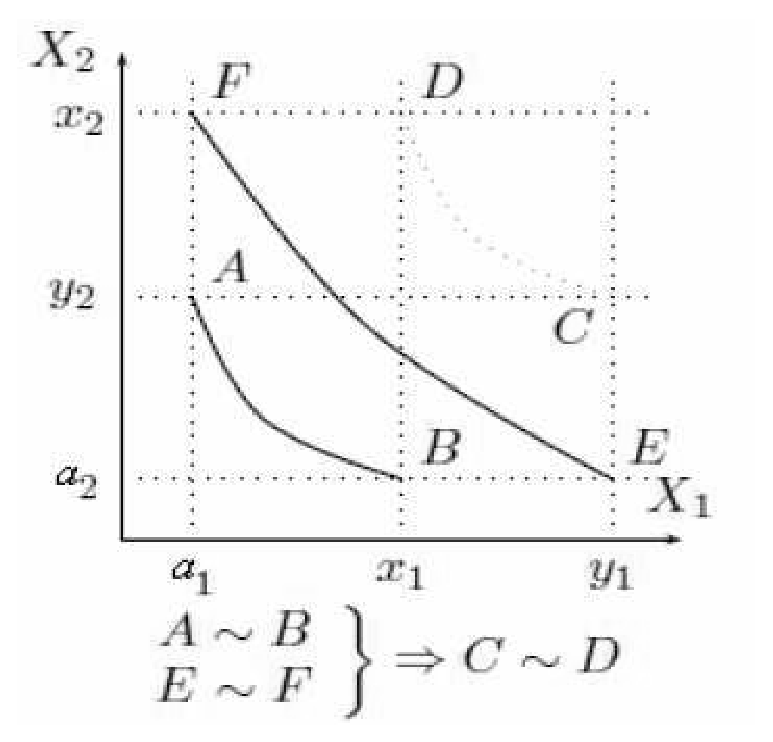
\includegraphics[scale=0.7]{thomsen}
%\\
%\end{center}
%\paragraph{Megfelelő trade-off értékek feltétel}
%kielégíthető, ha $\forall x_1, y_1, a_1, b_1 \in X_1$ és $\forall x_2, y_2, a_2, b_2 \in X_2$-re teljesül: 
%\begin{equation}
%(x_1, a_2) \sim (y_1, b_2) \text{ és } (a_1, a_2) \sim (b_1, b_2) \text{ és } (a_1, x_2) \sim (b_1, y_2)  
%\Rightarrow
%(x_1, x_2) \sim (y_1, y_2)
%\end{equation} 
%Ennek a feltételnek a teljesülése és a fent megadott kölcsönös preferenciafüggetlenség teljesülése elégséges és szükséges feltétele az additív értékelőfüggvény létezésének. Ez már jó.

Visszatérve nem kétdimenziós esetre, ott azért elegendő a kölcsönösen preferenciafüggetlenség, mert azokban az esetekben ez \textbf{páronként teljesíti az egyszerűsítési feltételt, ami pedig garantálja a páronkénti Thomsen feltételt}.

\subsection{Kvázi additív értékelő függvények}
Legyen $a=(x_1, ... , x_n) \in A$. Ekkor a preferencia struktúra \textbf{kvázi additív} $\Leftrightarrow$ teljesül: 
\begin{equation}
\begin{split}
v(a) = & \sum_{i=1}^n k_i \cdot v_i(x_i)+ \\
&\sum_{i=1}^n \sum_{j>i}^n k_{ij} \cdot v_i(x_i) \cdot v_j(x_j) + \\
&\sum_{i=1}^n \sum_{j>i}^n \sum_{l>j}^n k_{ijl} \cdot v_i(x_i)\cdot v_j(x_j)\cdot v_l(x_l) + ... \\ 
&+k_{1..n}\cdot v_1(x_1)\cdot  ... \cdot  v_n(x_n). \\
\end{split}
\end{equation} 
\paragraph{A kvázi additív alak jó tulajdonságai: }
\begin{enumerate}
\item Legyen $\sum_ik_{i} = 1$ és $k_{ij} = 0$, ... , $k_{1..n} = 0$. Ekkor pontosan az additív alakot fogjuk kapni.
\item  Legyen $k_{i} > 0$ és $k_{ij} = K\cdot k_{i}\cdot k_{j}$, ... , $k_{1..n} = K^{n-1}\cdot k_{1}\cdot ...\cdot k_{n}$. Ekkor a kvázi additív alak a következőképpen alakul:
\begin{equation}
\begin{split} 
v[v_1(x_1), ..., v_n(x_n)] = & \sum_{i=1}^n k_i\cdot v_i(x_i)+ \\
&+ K\cdot \sum_{i=1}^n \sum_{j>i}^n k_{i}\cdot k_{j}\cdot v_i(x_i)\cdot v_j(x_j) + \\
&+ K^{2}\cdot \sum_{i=1}^n \sum_{j>i}^n \sum_{l>j}^n k_{i}\cdot k_{j}\cdot k_{l}\cdot v_i(x_i)\cdot v_j(x_j)\cdot v_l(x_l) + \\
&+ ...  + K^{n-1}\cdot k_{1}\cdot ...\cdot k_{n}\cdot v_1(x_1)\cdot  ... \cdot  v_n(x_n) .\\
\end{split}
\end{equation} 
Ezt tekintsük egy egyenletnek, megszorozzuk mindkét oldalról $K$ majd hozzáadunk 1-et:
\begin{equation}
\begin{split} 1 + K \cdot  v[v_1(x_1), ..., v_n(x_n)] = & 1 + K \cdot \sum_{i=1}^n k_i\cdot v_i(x_i)+ \\
&+ K^2\cdot \sum_{i=1}^n \sum_{j>i}^n k_{i}\cdot k_{j}\cdot v_i(x_i)\cdot v_j(x_j) + \\
&+ K^{3}\cdot \sum_{i=1}^n \sum_{j>i}^n \sum_{l>j}^n k_{i}\cdot k_{j}\cdot k_{l}\cdot v_i(x_i)\cdot v_j(x_j)\cdot v_l(x_l) + \\
&+ ... + K^{n}\cdot k_{1}\cdot ...\cdot k_{n}\cdot v_1(x_1)\cdot  ... \cdot  v_n(x_n)  \\
\end{split}
\end{equation} 

Ekkor szorzattá alakítható (ha nem hiszed, próbáld ki a kéttényezős esetet!), majd átrendezhető:
\begin{equation}
\begin{split}
1 + K \cdot  v[v_1(x_1), ..., v_n(x_n)]  & = [1+K\cdot k_{1}\cdot  v_1(x_1)]\cdot ...\cdot [1+K\cdot k_{n}\cdot  v_n(x_n)] \\
v[v_1(x_1), ..., v_n(x_n)]  & = \frac{1}{K}([1+K\cdot k_{1}\cdot  v_1(x_1)]\cdot ...\cdot [1+K\cdot k_{n}\cdot  v_n(x_n)] - 1)
\end{split}
\end{equation} 
Ez a szorzat megfelel a multiplikatív alakkal.
\end{enumerate}


\paragraph{Def:} Egy $v: A \rightarrow \mathbb{R}$ \textbf{mérhető} $\Leftrightarrow v$ tükrözi \textbf{(1)} az $A$-beli elemek sorrendjét és \textbf{(2)} az elemek különbségeinek a sorrendjét. 

A mérhető $v$ létezésének vizsgálata nehézkes (itt most nem térünk ki rá).

Differenciaképzés: $\circ$.

\textbf{Mérhetőség feltétele:} $v$ mérhető, ha $\forall a,b,c,d \in A: a \circ b \succeq^* c \circ d$ $\Leftrightarrow$ $v(a)-v(b) \geq v(c)-v(d)$ 
 
 
\paragraph{Definíció: } Legyen $T=(X_1,...,X_m)$ tényezőhalmaz, $C \subseteq T$ gyenge differencia-független $C^*\subseteq T $-tól $\Leftrightarrow$ ha $\forall w_C,x_C,y_C,z_C \in X_C:$ valamely $w_{C^*}^0 \in X_{C^*}$ esetén teljesül minden más $w_{C^*} \in X_{C^*}$ -re, hogy: $(w_C, w_{C^*}^0) \circ (x_C, w_{C^*}^0) \succeq^* (y_C, w_{C^*}^0) \circ (z_C, w_{C^*}^0)$  $\Rightarrow$ $(w_C, w_{C^*}) \circ (x_C, w_{C^*}) \succeq^* (y_C, w_{C^*}) \circ (z_C, w_{C^*})$ 

\paragraph{Kvázi additivitási tétel} Tegyük fel, hogy
\begin{itemize}
\item létezik $v$ mérhető értékelő függvény
\item a legkevésbé preferált $a^0: v(a^0) = 0$ és a legjobban preferált $a^1: v(a^1)=1$
\item hasonlóan $\forall i \in 1,..,n : $ a legkevésbé preferált $x_i^0: v_i(x_i^0) = 0$ és a legjobban preferált $x_i^1: v_i(x_i^1)=1$.
\end{itemize}
Ha $\forall i \in 1,..,n : X_i$ tényező gyenge-differenciafüggetlen a komplementerhalmazától, akkor \textbf{$v$ felírható kvázi additív alakban}.

\subsection{Multiplikatív értékelő függvények}
Legyen $a=(x_1, ... , x_n) \in A$. Ekkor a preferencia struktúra \textbf{multiplikatív} $\Leftrightarrow$ teljesül:
\begin{equation}
\begin{split}
v(a)  & = \frac{1}{K}([1+K\cdot k_{1}\cdot  v_1(x_1)]\cdot ...\cdot [1+K\cdot k_{n}\cdot  v_n(x_n)] - 1)
\end{split}
\end{equation}

A multiplikatív alak létezéséhez (kettőnél nagyobb dimenziós esetben) a kölcsönös preferenciafüggetlenség helyett elegendő a következő feltétel: $\exists i$ index, amelyre $C=\{X_i\}$ tényezőrészhalmaz gyenge differencia független a komplementerétől és ugyanez az i index mellett teljesül, hogy $\forall j=1,...,n , j \neq i : C^{'}=\{X_i, X_j\}$ preferenciafüggetlen a komplementerétől. Ez könnyebben teljesül az additív alak létezési feltételénél, de szigorúbb a kvázi-additív alakénál.

\paragraph{$K$ skálázási konstans meghatározása 2D ($n=2$) esetben:}
\begin{equation}
\begin{split}
v(a) = & k_1\cdot v_1(x_1) + k_2\cdot v_2(x_2)+ \\
&K\cdot  k_{1}\cdot v_1(x_1)\cdot k_{2}\cdot v_2(x_2) \\
\end{split}
\end{equation}
Fejezzük ki $K$-t a $k_i$-kből, legyen $K = \dfrac{1 - (k_1 + k_2)}{k_1\cdot k_2}$. Ekkor:
\begin{equation}
\begin{split}
v(a) = & k_1\cdot v_1(x_1) + k_2\cdot v_2(x_2)+ \\
&\dfrac{1 - (k_1 + k_2)}{ \cancel{k_1\cdot k_2} } \cdot   \cancel{k_{1}}\cdot v_1(x_1)\cdot  \cancel{k_{2}}\cdot v_2(x_2) \\
= & k_1\cdot v_1(x_1) + k_2\cdot v_2(x_2)+ [1 - (k_1 + k_2)]\cdot v_1(x_1)\cdot v_2(x_2) \\
\end{split}
\end{equation}
Ahol az alábbi 3 eset állhat elő:
\begin{enumerate}
\item eset: $k_1 = 0$ és $k_2 = 0 \Rightarrow v(a) = v_1(x_1) \cdot  v_2(x_2), K \rightarrow \infty$. Konjukció, ÉS operátor. 
\item eset: $k_1 = 1$ és $k_2 = 1 \Rightarrow v(a) = v_1(x_1) + v_2(x_2) - v_1(x_1)\cdot  v_2(x_2), K = -1$. Diszjunkció, VAGY operátor.  
\item eset: $k_1 + k_2 = 1 \Rightarrow v(c) = k_1\cdot v_1(x_1) + k_2\cdot v_2(x_2), K = 0 $. Átlag művelet. (Additív alak)
\end{enumerate} 

A $k_i$-k tekinthetőek az adott tényezőhöz tartozó súlyozásként, a $K$ pedig azért felelős többek között, hogy az értékelés a $[0,1]$ intervallumba skálázódjon. A fentiek alapján a $K$ a $[-1, \infty]$ intervallumról vesz fel értéket. Ez határérték vizsgálatokkal kettőnél több tényezős esetben is belátható.


\subsection{Értékelő függvények megkonstruálása}

\paragraph{Jelölések:}

\begin{center}
\begin{tabular}{c||c|c|c|c|c}
 $A$ & $X_1$& $X_2$& $X_3$& $X_4$& $X_5$ \\
 \hline
 $a_1$&$v_1(x^{(1)}_{1})$  &$v_2(x^{(1)}_{2})$ & $v_3(x^{(1)}_{3})$ & $v_4(x^{(1)}_{4})$& $v_5(x^{(1)}_{5})$ \\
 $a_2$&$v_1(x^{(2)}_{1})$  &$v_2(x^{(2)}_{2})$ & $v_3(x^{(2)}_{3})$ & $v_4(x^{(2)}_{4})$& $v_5(x^{(2)}_{5})$ \\
 $a_3$&$v_1(x^{(3)}_{1})$  &$v_2(x^{(3)}_{2})$ & $v_3(x^{(3)}_{3})$ & $v_4(x^{(3)}_{4})$& $v_5(x^{(3)}_{5})$ \\
\end{tabular}
\end{center}
Ezekből meg szeretnénk kapni a $v(a_1), v(a_2), v(a_3)$-kat. Ez így többtényezős alak, ha az egyes $v_i(x^{(j)}_{i})$-ket tekintjük, akkor pedig az egytényezős értékelő függvényeket vizsgáljuk.

\subsubsection{Többtényezős értékelőfüggvény}

\paragraph{Hipotézisek alakra vonatkozó tesztekből:} 

\begin{itemize}
\item Kölcsönös preferenciafüggetlenség (2D esetben Thompsen feltétel) vagy a páronkénti Thompsen feltétel teljesülése $\Rightarrow$ additív alak
\item Kölcsönös gyenge differenciafüggetlenség és kritériumpárokra nézve kölcsönös preferenciafüggetlenség  $\Rightarrow$ multiplikatív forma
\item  Kölcsönös gyenge differenciafüggetlenség $\Rightarrow$ kvázi additív forma
\item Minden más esetben  $\Rightarrow$ egyéb formák

\end{itemize}

\paragraph{Konstruálás: }

\begin{enumerate}
\item Többtényezős értékelőfüggvény létezésének verifikálása. Pl: teljesül-e a preferencia struktúrára a gyenge rendezés tulajdonságai. Ha nem teljesül, akkor rossz a preferencia struktúra, megkérjük a döntéshozót, hogy racionális preferencia struktúrát állítson fel. %Ha nem ismert a preferencia struktúra, akkor feltesszük, hogy létezik: megköveteljük a függvénytől a monotonitást, és folytonosságot.
\item Megfelelő alakú függvényforma kiválasztása. Főleg a (gyenge differencia, és preferencia, Thomsen) függetlenségi tesztek alapján történik. Mivel ezek közül csak a preferencia függetlenség ellenőrizhető intuitíven, ezért általában multiplikatív alak használata javasolt.
\item Az összetevő egydimenziós értékelő függvények megkonstruálása. (\ref{sssec:1D}.-ban bemutatottak alapján)
\item Konstansok kiválasztása: Kellő mennyiségű preferencia információ alapján felírunk egy konstansokra vonatkozó független egyenletrendszert, megoldjuk. (Konkrét megvalósítással nem foglalkozunk, hasonló a multiplikatív konstansok beállításához.)
\item Konzisztencia ellenőrzés, elemzés. (Döntéshozóval együtt, kérdezéses módszerrel)
\end{enumerate}

\subsubsection{Egydimenziós értékelőfüggvény}
\label{sssec:1D}
\begin{enumerate}

\item \textbf{A döntéshozó direkt értékelést ad.} Általában nem tud, nehéz, nem lesz konzisztens. (Az elemi módszereknél ezzel próbálkoztunk).

\item \textbf{Lineáris értékelő függvény:} meghatározzuk az adott tényező szélső értékeit és a közötte lévő részt egyszerűen behúzzuk egy egyenessel.

Ennek a módszernek az alapján lehetséges bármely más görbe használata is (például szigmoid).

\item \textbf{Felező módszer:}
Az eljárást minden $X_k \in X$ tényezőre végrehajtjuk:
\begin{enumerate}
\item Adjunk meg egy egyértelmű rendezést a lehetséges tényező értékek felett.
\item Válasszuk ki a legkevésbé kívánatos $x^0_k $ és a leginkább kívánatos $x^1_k$ tényezőértéket. A valós értéküket rögzítsük: $v(x^0_k) = 0 $, $v(x^1_k) = 1$
\item Amíg nem találjuk meg a $x^0_k$ és a $x^1_k$ középpontját, vegyünk egy tetszőleges $x^\prime_k \in X_k$ tényezőértéket és kérdezzük meg a döntéshozót, hogy értékelje a $x^0_k$-ből és a $x^1_k$-ből való elmozdulást a vizsgált tényezőérték esetében. Ha a két elmozdulás között eltérés van, akkor vegyünk egy további tényezőértéket abból az intervallumból, ahol a középpont várhatóan megtalálható lesz. Ha megvan akkor $ v(x^{0.5}_k) = v(x^{\prime}_k) = 0.5$ és ekkor léphetünk a következő lépésre.
\item Az előző lépés alkalmazása a $x^0_k$ és a $x^{0.5}_k$ közötti $x^{0.25}_k$ és a $x^{0.5}_k$ és a $x^1_k$ közötti $x^{0.75}_k$ középpont megtalálásáért.
\item Konzisztencia ellenőrzés: a kapott $x^{0.25}_k$ és $x^{0.75}_k$ középpontja valóban a $x^{0.5}_k$?
\item Ismételjük a (c) lépéstől, a részletezni kívánt intervallumon, addig míg elegendő pont nem lesz a görbe illesztéséhez. A görbének rendelkeznie kell a korábban vizsgált tulajdonságokkal (folytonosság, monotonitás)
\end{enumerate}

\end{enumerate}

\begin{center}

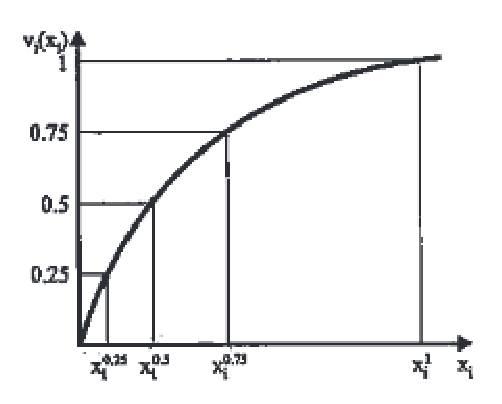
\includegraphics[scale=0.7]{valuesample}
\\
\end{center}

%Hasonló példa: számkitalálós játék: algoritmus: mindig felezzük az ismert intervallumot.

\section{Döntés bizonytalanság mellet (sztochasztikus modellek)}

Sztochasztikus döntési modell esetében a vizsgálat értékeink kibővülnek a természet egyes állapotainak valószínűségével ($s_k$). \textbf{Kockázatos döntések.}

\paragraph{Feladat:} Tegyük fel, hogy rendelkezünk 35 millió forinttal, melyet szeretnénk úgy befektetni, hogy a lehető legnagyobb hozamunk legyen a következő 5 évre. Bizonytalan eseményként vizsgáljuk az infláció alakulását.

A feladat egyszerűsége kedvéért két lehetőség közül választunk: ingatlan befektetés ($a_1$) vagy infláció követő állampapír ($a_2$). Mindkét esetben a teljes összeget elköltjük a befektetésre. A feladat során az infláció alakulása alapján vizsgáljuk, hogy mennyi pénzünk lesz a vizsgált az időszak végére.

Az államkötvény esetében tegyük fel, hogy 0.25$\%$ kamatprémiumot fizet az infláción felül (az adott évben mindig az eggyel korábbi év inflációjára számoljuk ezt). Az éves lakbér legyen az adózás után az ingatlan vásárlási értékének a 3.4$\%$-a (1.2 millió forint). Tegyük fel, hogy a lakbér adózáson kívül nincs további költsége az ingatlan üzemeltetésének. Továbbá az egyszerűség kedvéért tegyük fel, hogy a megkapott kamatot illetve lakbért nem fektetjük be újra.

Az infláció lehetséges alakulása:
\begin{center}
\begin{tabular}{c||r|r|r|r|r|r|}
      & 2022 & 2023  & 2024  & 2025 & 2026  \\
 \hline
 $s_1$&14.5$\%$&18.4$\%$& 9$\%$ & 9$\%$ & 7$\%$\\
 $s_2$&14.5$\%$&17.4$\%$& 6$\%$ & 4.5$\%$ & 3.5$\%$ \\

\end{tabular}
\end{center}

Az államkötvény esetén 9 év utána az eredeti összeget kapnánk vissza, viszont mivel jelen esetben a 5 év után visszaváltjuk (a jelenlegi visszaváltási feltételt feltételezve) ezért az eredeti összeg 1$\%$-kal csökkentett értékét kapjuk (az 5. év forduló nap előtti utolsó nap visszaváltva az utolsó évi kamat minusz 1$\%$-kal számolhatunk). A lakást ugyanígy 5 év múlva értékesítjük, így ebben az esetben is további hozamhoz juthatunk. Amennyiben az infláció tartósan magas marad ($s_1$), akkor ehhez jó eséllyel a magas kamatkörnyzet, drága lakáshitelek és a történelmi példák alapján a lakásárak oldalazására lehet számítani. Tehát ebben az esetben ugyanannyiért tudjuk eladni, mint amennyiért megvettük. A másik esetben ($s_2$), ha az infláció a vizsgált 5 év végére mérséklődik, akkor az első évek oldalazása után egy hirtelen 50$\%$-os emelkedés várható.

Az ingatlant továbbá olyan szerződéssel szeretnénk bérbe adni, amelyben garantáltan az előző évi infláció mértékében növekvő lakbért várunk el. A második esetben ($s_2$) sikerül ilyen bérlőt találnunk, akinek megfelel a feltétel. Viszont amennyiben tartósan magas marad az infláció, akkor nem sikerül ilyen szerződést kötnünk és nem nőnek a lakásárak sem. Így ebben az esetben végig a kezdő 3.4$\%$-kal számolunk.


Ezeket összegezve az infláció lehetséges alakulása mellett az éves bevételeink a befektetés százalékában:
\begin{center}
\begin{tabular}{c c||r|r|r|r|r||r}
    &  & 2023& 2024  & 2025  & 2026 & 2027 & összesen \\
 \hline
 $s_1$&$a_1$&3.40$\%$&3.40$\%$&3.40$\%$&3.40$\%$&3.40$\%$ & 17.00$\%$ \\
 $s_2$&$a_1$&3.89$\%$&4.57$\%$&4.84$\%$&5.06$\%$&55.24$\%$ & 73.60$\%$ \\
 \hline
 $s_1$&$a_2$&14.75$\%$&18.65$\%$&9.25$\%$ & 9.25$\%$& 6.25 $\%$ & 58.15$\%$ \\
 $s_2$&$a_2$&14.75$\%$&17.65$\%$&6.25 $\%$ & 4.75$\%$ & 2.75 $\%$ & 46.15$\%$ \\

\end{tabular}
\end{center}



%\paragraph{Feladat:} Rendelkezünk 10 millió forint befektetésre szánt pénzzel, melyet szeretnénk úgy befektetni, hogy a lehető legnagyobb reálhozamunk legyen. Bizonytalan eseményként vizsgáljuk az infláció alakulását.

%Magas infláció mellett történelmi adatok alapján érdemes bankok részvényeit megvásárolni. A történelmi adatokon kívül könnyen számolható éves nyereséget okoz a bankok számára a magas %inflációs környezet. Egyik lehetséges alternatívánk, hogy megvesszük a rendelkezésre álló keretből egyetlen, tetszőleges bank részvényét. A jelenlegi feladatban feltesszük, hogy kezdő %tőzsdei befektetők vagyunk, nem diverzifikálunk, egyetlen vásárlás. Ennek köszönhetően valami benyomás alapján választunk egy bankot. Ebből fakadóan tegyük fel, hogy nem sikerült a %legjobban teljesítő bank részvényét kiválasztani, illetve hogy magas áron sikerült megvenni a részvényt. Ennek eredményeképpen alacsonyabb inflációs környezet esetén az első évben 10$\%%$-ot veszítünk, míg ha az infláció tartósan magas lesz, akkor a kalkulációink alapján várhatóan éves szinten 20$\%$ reálnyereségünk lehet (inflálódást, mindenféle utalási, %részvényvásárlási, adózási költséget mindkét esetben beleszámítva, illetve a különböző valutaváltási és valutánként eltérő infláció mértékkel, vagy bármi további részlettel a feladat %egyszerűsítése kedvéért most nem foglalkozunk).
%
%A másik lehetséges alternatívánk a Magyar Állampapír Plusz megvásárlása, amely 5 évre 4.95$\%$ kamatot tud nyújtani. Amennyiben 5$\%$ körüli magas infláció lesz, akkor az első évben %0.05$\%$-os reálérték veszteségünk lesz, míg amennyiben az infláció mérséklődik 2$\%$ körüli szintre, akkor 2.95$\%$ reálhozamunk lehet.
%
%Melyik befektetést válasszuk?
%
%\begin{center}
%\begin{tabular}{l|c|c}
%\multirow{2}{*}{\bf Cselekvési lehetőségek } &  \multicolumn{2}{c}{ \bf Események }\\
% & $s_1=$ magas infláció (5$\%$) & $s_2=$ alacsony infláció (2$\%$) \\
%\hline
%  $a_1=$ egy bank részvény & 12 & 9 \\
%  $a_2=$ MÁP & 9.995 & 10.295 \\
%\end{tabular}
%\end{center}
%$P(s_1) = 0.55 , P(s_2) = 0.45$ szubjektív valószínűségi értékek (becslések).


%\paragraph{Feladat:} Befektetési feladat: rendelkezünk 12 millió forint befektetésre szánt pénzzel. Két befektetési lehetőségen gondolkozunk: vehetünk belőle 10 ha jó minőségű termőföldet, vagy az aktuális alapkamaton elérhető banki lekötést választjuk.

%A termőföld vásárlása esetén egyrészt a termőföld éves bérbeadásából származó nyereséget könyvelhetjük el, másrészt a jó minőségéből és a piaci környezetből adódóan évről-évre folyamatosan emelkedik az értéke. A példában egy év alatt 2 millió forint nyereség várható.

%A környéken nem megoldott a kellő hulladékkezelés. Ennek köszönhetően várhatóan egy hulladéklerakó fog létesülni a termőföldünk szomszédságában. A beruházásra nincs meg a kellő forrás. A helyi önkormányzat ezt a forráshiányt a kellő biztonsági intézkedéseken spórolná meg, így a híg hulladéklé a termőföldünkön folyna keresztül és összességében 90$\%$-kal esne vissza a termőföldünk értéke és a termés is tönkremegy (nem lesz belőle bevételünk). A rendelkezésre álló információk alapján 25$\%$-ra becsüljük annak a valószínűségét, hogy a hulladéklerakó megépül. 

%Ugyanakkor lelkes helyi civilek aláírásgyűjtésbe kezdenek a hulladéklerakó távolabbra és biztonságosabb elhelyezésért. Ha a kezdeményezés sikeres akkor ebben az esetben nem valósulna meg a beruházás. Mivel a környék eleve forráshiánnyal kűzd ezért ennek az esetnek (hulladéklerakó nem megépülése) szerintünk 75$\%$ a becsült esélye. 

%A másik lehetőségünk, hogy banki lekötésbe fektetjük a pénzünk. Ha ez mellett nem lesz új beruházás (hulladéklerakó) számolnunk kell azzal, hogy a jelenlegi 3.8$\%$-os alapkamatot az MNB tovább vágja 3$\%$-ra, ami érinti a banki lekötésünket. Ellenkező esetben marad a kamatszint.

%\begin{center}
%\begin{tabular}{l|c|c}
%\multirow{2}{*}{\bf Cselekvési lehetőségek } &  \multicolumn{2}{c}{ \bf Események }\\

% & $s_1=$ hulladéklerakó épül & $s_2=$ nincs új beruházás \\
%\hline
%  $a_1=$ termőföldvásárlás & -10 800 & 2 000 \\
%  $a_2=$ pénz a bankban & 456 & 360\\
%\end{tabular}
%\end{center}
%$P(s_1) = 0.25 , P(s_2) = 0.75$ szubjektív valószínűségi értékek (becslések).

Melyik befektetést válasszuk?

\begin{center}
\begin{tabular}{l|c|c}
\multirow{2}{*}{\bf Cselekvési} &  \multicolumn{2}{c}{ \bf Események }\\
 {\bf lehetőségek} & $s_1=$ tartósan & $s_2=$ enyhülő \\
  & magas infláció &  infláció \\
\hline
  $a_1=$ ingatlan vásárlás & 40.95 & 60.76 \\
  $a_2=$ PMÁP & 55.35 & 51.15 \\
\end{tabular}
\end{center}
$P(s_1) = 0.55 , P(s_2) = 0.45$ szubjektív valószínűségi értékek (becslések).

\subsection{Dominancia módszer}
\label{susec:domi}
Amennyiben egy alternatíva minden esemény bekövetkezése esetén jobb értékekkel rendelkezik, mint egy másik, akkor dominálja azt és a dominált alternatíva elhagyható.

A fenti példában nincs ilyen alternatíva.

\subsection{Döntés a pénzérték alapján}
\label{susec:penzert}
A döntésben csak a nyereségértékeket vesszük figyelembe a valószínűségeket nem.
\paragraph{Pesszimista, maximin kritérium:}  sorminimumok maximuma $\rightarrow a_2$
\paragraph{Optimista, maximax kritérium:}  sormaximumok maximuma $\rightarrow a_1$

\

De pénzérték alapján ezen enyhíteni szoktak $\rightarrow$ optimizmus együttható: \emph{Hurwick-féle} $\alpha$, a döntéshozó $\alpha$ arányban optimista és $1-\alpha$ arányban pesszimista. Legyen például $\alpha \gets 0.8$, ekkor a példánkban: 
\begin{center}
$H_{a_1} \gets 0.8\cdot 60.76 + 0.2\cdot 40.95 = 56.798$
%$H_{a_1} \gets 0.8\cdot 60.59 + 0.2\cdot 40.95 = 56.662$
%$H_{a_1} \gets 0.8\cdot 2000 + 0.2\cdot -10800 = -560$

$H_{a_2} \gets 0.8\cdot 55.35 + 0.2\cdot 51.15 = 54.51$
%$H_{a_2} \gets 0.8\cdot 57.58 + 0.2\cdot 52.50 = 56.564$
%$H_{a_2} \gets 0.8\cdot 456 + 0.2\cdot 360 = 436.80$
\end{center}

A döntést a $max\{H_{a_1},H_{a_2}\}$ alapján hozzuk, így az $a_1$-et választjuk.

\subsection{Döntés a valószínűségérték alapján}
\label{susec:vaert}
\paragraph{Maximum likelihood kritérium: } azt választjuk, amelynek a legnagyobb a bekövetkezési valószínűség mellett legnagyobb a pénzértéke. 

Tehát a $P(s_1)$-nek a legnagyobb a valószínűsége, így az $a_2$-t választjuk.

\subsection{Döntés a várható pénzérték alapján}
\label{VP}
Alternatívánként vesszük a természet állapotaihoz tartozó várható pénzértéket és azok valószínűségét. Kiszámoljuk az állapotok becsült valószínűségekkel súlyozott összegeit és kiválasztjuk közülük a maximálisat.

$VP(a_1) = 0.55\cdot 40.95 + 0.45\cdot 60.76 = 49.8645$
%$VP(a_1) = 0.55\cdot 40.95 + 0.45\cdot 60.59 = 49.788$
%$VP(a_1) = 0.25\cdot -10800 + 0.75\cdot 2000 = -1200$

$VP(a_2) = 0.55\cdot 55.35 + 0.45\cdot 51.15 = 53.46$
%$VP(a_2) = 0.55\cdot 57.58 + 0.45\cdot 52.50 = 55.294$
%$VP(a_2) = 0.25\cdot 456 + 0.75\cdot 360 = 384$

Az $a_2$-t választjuk.


\subsection{Döntés az elmulasztott nyereség alapján}
\label{susec:elmunyer}
Ebben az esetben se vesszük figyelembe a valószínűségeket. Ugyanakkor a pénzérték helyett itt az adott esemény által elérhető maximális nyereségtől való eltérést vesszük. Ezek alapján a táblázatunk a következőképpen néz ki:

%\begin{center}
%\begin{tabular}{l|c|c}
%\multirow{2}{*}{\bf Cselekvési lehetőségek } &  \multicolumn{2}{c}{ \bf Események }\\
% & $s_1=$ hulladéklerakó épül & $s_2=$ nincs új beruházás \\
%\hline
%  $a_1=$ termőföldvásárlás  & 11 256 & 0 \\
%  $a_2=$ pénz a bankban & 0 & 1640\\
%\end{tabular}
%\end{center}

%\begin{center}
%\begin{tabular}{l|c|c}
%\multirow{2}{*}{\bf Cselekvési} &  \multicolumn{2}{c}{ \bf Események }\\
% {\bf lehetőségek} & $s_1=$ tartósan & $s_2=$ enyhülő \\
%  & magas infláció &  infláció \\
%\hline
%  $a_1=$ ingatlan & 19.64 & 0 \\
%  $a_2=$ PMÁP & 3.01 & 8.09 \\
%\end{tabular}
%\end{center}

\begin{center}
\begin{tabular}{l|c|c}
\multirow{2}{*}{\bf Cselekvési} &  \multicolumn{2}{c}{ \bf Események }\\
 {\bf lehetőségek} & $s_1=$ tartósan & $s_2=$ enyhülő \\
  & magas infláció &  infláció \\
\hline
  $a_1=$ ingatlan & 19.81 & 0 \\
  $a_2=$ PMÁP & 5.41 & 9.61 \\
\end{tabular}
\end{center}

\paragraph{Pesszimista döntéshozó:} A döntést az alternatívánkénti (soronkénti) maximális értékek minimuma fogja adni. Tehát az $a_2$-t választjuk.

\subsection{Döntés a várható elmulasztott nyereség alapján}
Az előzővel teljesen azonosan, azt leszámítva, hogy az elmulasztott nyereség táblázatából vesszük az értékeket és itt a minimálisat választjuk.

$VE(a_1) = 0.55\cdot 19.81 + 0.45\cdot 0 = 10.8955$

$VE(a_2) = 0.55\cdot 5.41 + 0.45\cdot 9.61 = 7.3$

Az $a_2$-t választjuk.

\subsection{Döntés a rendelkezésre álló információ alapján}
Azonos a \ref{VP} szekcióban bemutatottakkal, várható pénzértéket számolunk. Annyival bővül, hogy itt kihangsúlyozzuk azt, hogy a valószínűségeket \emph{rendelkezésre álló információnak} tekintjük. Tehát azok szubjektív valószínűségek.

%$VPRI(a_1) = 0.25\cdot -10800 + 0.75\cdot 2000 = -1200$
%$VPRI(a_1) = 0.55\cdot 12 + 0.45\cdot 9 = 10.65$
%$VPRI(a_1) = 0.55\cdot 40.95 + 0.45\cdot 60.59 = 49.788$
$VPRI(a_1) = 0.55\cdot 40.95 + 0.45\cdot 60.76 = 49.8645$

%$VPRI(a_2) = 0.25\cdot 456 + 0.75\cdot 360 = 384$
%$VPRI(a_2) = 0.55\cdot 9.995 + 0.45\cdot 10.295 = 10.13$
%$VPRI(a_2) = 0.55\cdot 57.58 + 0.45\cdot 52.50 = 55.294$
$VPRI(a_2) = 0.55\cdot 55.35 + 0.45\cdot 51.15 = 53.46$

%$VPRI = max\{VPRI(a_1), VPRI(a_2)\} = 10.65$
$VPRI = max\{VPRI(a_1), VPRI(a_2)\} = 53.46$

\subsection{A tökéletes információ várható pénzértéke} 
Ha élne egy jós, aki meg tudná mondani, hogy milyen lesz az infláció, %elindul-e a beruházás,
akkor ennek az információnak mekkora a várható pénzértéke?
(Mennyit érdemes fizetni a tökéletes információért cserébe?)
Feltevés: a jós által mondott esemény biztosan bekövetkezik.

Első lépésben meg kell vizsgálni, hogyha az általunk ismert eseményeket állítja a jós, akkor azokat biztosan bekövetkező eseményként vizsgálva mekkora a várható pénzérték.
Itt azért szerepel továbbra is egy valószínűségi súlyozás, mert így ad teljes eseményteret a két eset. Ennek olyan jelentése van, hogy szerintünk ekkora valószínűséggel mondja a jós, hogy $s_{i}$ esemény következik be biztosan. Ez megegyezik a korábbi valószínűséggel ugyanis a két esemény bekövetkezéséről továbbra is ez a véleményünk. Amennyiben a jós bevonása ezen változtatna, akkor ez természetesen módosulhat.

Lehetséges előrejelzés:
\begin{itemize}
\item ha $s_{1}$ lesz a jós szerint $\rightarrow$ optimális cselekvés: $a_2$  és a $VP(a_1) = 0.55\cdot 55.35 = 30.4425$
\item ha $s_{2}$ lesz a jós szerint $\rightarrow$ optimális cselekvés: $a_1$  és a $VP(a_2) = 0.45\cdot 60.76 = 27.342$
\end{itemize}

A tökéletes információ várható pénzértéke ennek a két lehetőségnek az összege: 

$VPTI = 30.4425 + 27.342 = 57.7845$

"Mennyit fizessünk a jósnak?" kérdésre a válasz: $VPTI - VPRI = 57.7845 - 53.46 = 4.3245$ (ez egy maximum érték, ennél többet nem ér az információ)

\subsection{Döntés nem tökéletes információ alapján}
\label{sec:NTI}

Mivel ténylegesen tökéletes információval rendelkező jósok nem léteznek, ezért helyettük érdemesebb kockázatelemző, előrejelző céget keresni. Ami a következő állításokat teheti:
\begin{itemize}
\item $z_{1}:$ azt állítják (előrejelzik), hogy az infláció magasan marad.  %(általánosan: bekövetkezik vmely esemény, itt speciálisan, ez az $s_{1}$)
\item $z_{2}:$ azt állítják, hogy az infláció mérséklődik. % $s_{2}$ következik be (általánosan: nem következik be a $z_{1}$-ben feltett esemény, itt speciálisan, ez az $s_{2}$)
\end{itemize}

Tegyük fel, hogy a cégről ismert \textbf{az előrejelzési pontossága}, korábbi évek előrejelzéseinek a pontossága alapján:
\begin{itemize}
\item $P(z_{1}|s_1) = 0.8$ 
\item $P(z_{2}|s_1) = 1- P(z_{1}|s_1) = 0.2$
\item $P(z_{2}|s_2) = 0.7$ 
\item $P(z_{1}|s_2) = 0.3$ 
\end{itemize}
Ezek a \textbf{beválási valószínűségek (likelihoodok)}. Akár meg is egyezhetnének a $s_1$ és $s_2$-re, de általában a változás bekövetkezést nehezebb előre jelezni. Ez az információ a feladatok többségében elérhető, ennek elérhetősége az előfeltétele a feladat végrehajtásának. Az előző fejezetben például a jósnak 1 volt a találati értéke és 0 a tévesztési score-ja mindkét esetben.

Az ilyen feladatok esetében a $P(s_1) = 0.55 , P(s_2) = 0.45$ saját véleményen alapuló valószínűségi értékeket tekintjük \textbf{a priori valószínűségek}nek. 

\textbf{A Bayes-tétellel kiszámolható a posteriori valószínűségeket}: $P(s_1|z_1),$ $P(s_2|z_1),$ $ P(s_1|z_2),$ $P(s_2|z_2)$
\begin{equation}
\begin{split}
P(s_1|z_1) =& \frac{P(z_{1}|s_1) \cdot  P(s_1)}{\sum_{i}^{ } P(z_{1}|s_i) \cdot  P(s_i)} \\
&\vdots \text{ a többit hasnolóan} \\
\\
P(z_1)=\sum_{i}^{ } P(z_{1}|s_i) \cdot  P(s_i) =  0.8\cdot 0.55+0.3\cdot 0.45 &= 0.575 \\
P(z_2)=\sum_{i}^{ } P(z_{2}|s_i) \cdot  P(s_i) =  0.2\cdot 0.55+0.7\cdot 0.45 &= 0.425 \\
P(s_1|z_1) = \frac{0.44}{0.575} = 0.7652,  
P(s_2|z_1) = \frac{0.135}{0.575} &= 0.2348 \\
P(s_1|z_2) = \frac{0.11}{0.425} = 0.2588,
P(s_2|z_2) = \frac{0.315}{0.425} &= 0.7412
\\
\end{split}
\end{equation}

Ezekből pedig kifejezhető az adott alternatíva, adott előrejelzés melletti várható pénzértéke:

$VP(a_1|z_1) = \sum_{i}^{ }v(s_i,a_1)\cdot P(s_i|z_1) = 40.95\cdot 0.7652 + 60.76\cdot 0.2348 = 45.601388$ 
 
$VP(a_2|z_1) = \sum_{i}v(s_i,a_2)\cdot P(s_i|z_1) = 55.35\cdot 0.7652 + 51.15\cdot 0.2348 = \textbf{54.36384}$ 

$VP(a_1|z_2) = \sum_{i}v(s_i,a_1)\cdot P(s_i|z_2) = 40.95\cdot 0.2588 + 60.76\cdot 0.7412 = \textbf{55.633172}$  

$VP(a_2|z_2) = \sum_{i}v(s_i,a_2)\cdot P(s_i|z_2) = 55.35\cdot 0.2588 + 51.15\cdot 0.7412 = 52.23696$

\paragraph{A nem tökéletes információ várható pénzértéke: }

Ajánlatot kapunk az eddig vizsgált előrejelző cégtől: 1.5 millió forintért előrejelzést adnak az inflációra. A kérdés megéri-e ennyiért elfogadni az ajánlatot. Mennyit ér a nem tökéletes információ?

Lehetséges előrejelzés:
\begin{itemize}
\item $z_{1} \rightarrow$ optimális cselekvés: $a_2$  és a $VP(a_2) = VP(a_2|z_1) \cdot  P(z_1) = 54.36384\cdot 0.575 = 31.259208$
\item $z_{2} \rightarrow$ optimális cselekvés: $a_1$  és a $VP(a_1) = VP(a_1|z_2) \cdot  P(z_2) = 55.633172\cdot 0.425 = 23.6440981$
\end{itemize}

Nem teljes információhoz tartozó pénzérték: $VPNTI = \sum_{j} VP(a_j) = 31.259208 + 23.6440981 = 54.903$

A "Mennyit fizessünk legfeljebb az előrejelző cégnek?" kérdésre a választ az alábbiak alapján tudjuk megkapni: $VPNTI - VPRI = 54.90 - 53.46 = 1.44$. Ami egy maximális érték arra, amennyiért megéri őket alkalmazni. Mivel ez feletti ajánlat érkezett, ezért elutasítjuk.

\subsection{Döntés döntési fa eljárás alapján}

Kiértékelési eljárásnak fogható fel. A döntési fa struktúra itt egy absztrakciós szintként jelenik meg, ami segíti a $\ref{sec:NTI}$ fejezetben bemutatott "információ értéke" döntési feladat áttikenthetőségét. (Az itt tárgyaltak kizárólag a nevében egyeznek meg a döntési fa - gépi tanulási eljárással.)

A kérdés, amire a megoldást keressük egyrészről az, hogy melyik alternatívát válasszuk, másrészről pedig az, hogy igénybe vegyünk-e (a példában megadott mértékű) $d$ költségű előrejelzést. Tehát a feladat itt nem az információ értékének a kiszámítása, hanem a döntési folyamat egyes lépéseinek és egészének a várható pénzértékének a számítása, melyeket maximalizálni szeretnénk. Így ez megadja az optimális döntéseket az adott szituációkban.

Jelölésben, új cselekvési alternatívákat vezetünk be: 
\begin{itemize}
\item $e_{0}:$ nem veszünk igénybe előrejelzést (ekkor $z_{0}$ üres esemény fog megtörténni, $P(z_0) = 1$)
\item $e_{1}:$ igénybe vesszük az eddig vizsgált előrejelező céget (ennek a műveletnek $d$ költsége van)
\end{itemize}

\begin{center}

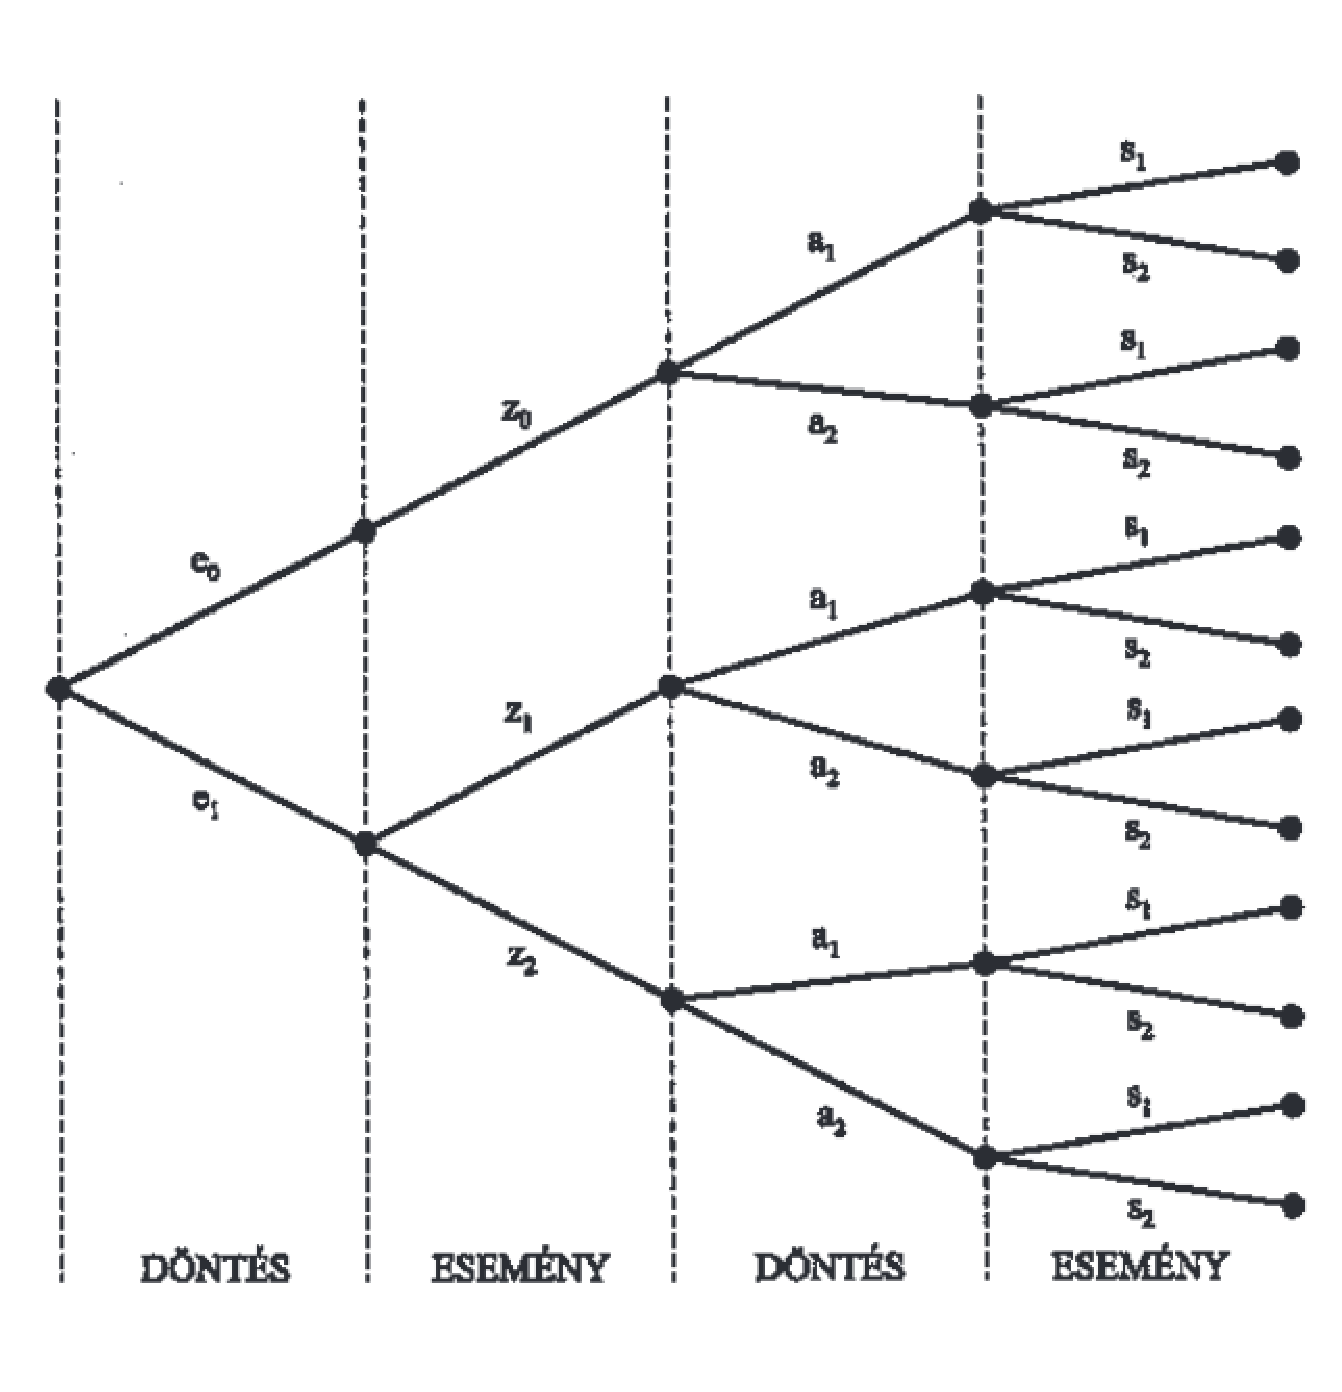
\includegraphics[scale=0.7]{dectree01}
\\
\end{center}

\paragraph{Előkészületek: }
\begin{itemize}
\item a fát a gyökérből indulva rajzoljuk meg, minden lehetséges döntésnek és lehetséges eseménynek külön ágat húzunk be (fenti ábra).
\item az eseményekhez tartozó valószínűségeket be tudjuk helyettesíteni az egyes ágakra. Egy esemény minél mélyebben van, annál több dologtól függ. A lentebbi ágakon a felette lévőekkel alkot feltételes valószínűséget. Pl: egy lentebbi ágon $P(s_1|z_1)$ van, míg felül $P(z_1)$ van (tehát ez utóbbi nem függ az $s_i$-től).
\item a levelekhez be tudjuk írni az egyes választások pénzértékét a táblázatból (előrejelzés esetében már itt $d$ = 1.5 millió forinttal terhelt pénzértékeket).
\end{itemize}

\paragraph{Eljárás: }
a levélből elindulva, felfelé propagálva kiszámoljuk az egyes csúcsokat ($K$ az aktuális csúcs):
\begin{itemize}
\item az események esetében kiszámoljuk a csúcshoz tartozó várható pénzértéket: \\
 $VP_K = \sum_{i\in K} ag_i\cdot gyerek_i$ 
\item döntési elágazás: kiválasztjuk a $max_{i\in K}\{gyerek_i\}$ és a nem maximális értékhez tartozó ágat levágjuk. Ez lesz a csúcs várható pénzértéke.
\end{itemize}

Végül a gyökérben egyetlen, a feladat várható pénzértéke marad és az ahhoz tartozó optimális döntések.

\begin{center}

\includegraphics[scale=0.7]{dectree05}
\\
\end{center}

\section{Multi-attribute utility theory --- Hasznosság függvény}
\label{sec:utility}

A MAUT egy általános összefoglaló neve a többtényezős hasznosság elméletnek, több tárgyalásban ebbe beleértik az értékelő függvényeket is (azt is hasznosságként kezelik). Az alapfeltevése az, hogy minden döntéshozó megpróbál optimalizálni egy olyan függvényt, amely aggregálja az összes véleményét az adott kérdésben. Ez azt feltételezi, hogy a döntéshozó racionális és optimalizáló szemléletű. (Ennek kritikájáról hallhattunk Ha-Joon Chang és Daniel Kahneman könyve nyomán tartott előadásokban)

%\paragraph{Jelölés:}
%\begin{center}
%\begin{tabular}{c|||c|c|c|c|c||c|c|c|c|c}
% \multirow{2}{*}{$A$} & \multicolumn{5}{c}{$s_1$ }& \multicolumn{5}{|c}{$s_2$ } \\
% & $X_1$& $X_2$& $X_3$& $X_4$& $X_5$ & $X_1$& $X_2$& $X_3$& $X_4$& $X_5$ \\
% \hline
% $a_1$&$x^{(1,1)}_{1}$  &$x^{(1,1)}_{2}$ & $x^{(1,1)}_{3}$ & $x^{(1,1)}_{4}$& $x^{(1,1)}_{5}$ & $x^{(1,2)}_{1}$  &$x^{(1,2)}_{2}$ & $x^{(1,2)}_{3}$ & $x^{(1,2)}_{4}$& $x^{(1,2)}_{5}$\\
% $a_2$&$x^{(2,1)}_{1}$  &$x^{(2,1)}_{2}$ & $x^{(2,1)}_{3}$ & $x^{(2,1)}_{4}$& $x^{(2,1)}_{5}$&$x^{(2,2)}_{1}$  &$x^{(2,2)}_{2}$ & $x^{(2,2)}_{3}$ & $x^{(2,2)}_{4}$& $x^{(2,2)}_{5}$ \\
% $a_3$&$x^{(3,1)}_{1}$  &$x^{(3,1)}_{2})$ & $x^{(3,1)}_{3}$ & $x^{(3,1)}_{4}$& $x^{(3,1)}_{5}$&$x^{(3,2)}_{1}$  &$x^{(3,2)}_{2})$ & $x^{(3,2)}_{3}$ & $x^{(3,2)}_{4}$& $x^{(3,2)}_{5}$ \\
%\end{tabular}
%\end{center}
%ahol, $A=\{a_1,a_2,a_3\}$ alternatívák halmaza, $X = \{X_1$, $X_2$, $X_3$, $X_4$, $X_5\} $ tényezők (kritériumok) halmaza, $S = \{s_1,s_2\}$ vizsgált bekövetkezhető események, és $x^{(j,k)}_{i}$ lehetséges kimenetelek, amiket tényezőértékek jelölnek.


%\paragraph{Jelölés rövidebben:}
%\begin{center}
%\begin{tabular}{c||c|c}
% $A$ & $s_1$ & $s_2$ \\
% \hline
% $a_1$&$c^{(1,1)}$  &$c^{(1,2)}$ \\
% $a_2$&$c^{(2,1)}$  &$c^{(2,2)}$ \\
% $a_3$&$c^{(3,1)}$  &$c^{(3,2)}$ \\
%\end{tabular}
%\end{center}
%ahol $c^{(1,1)} = $[$x^{(1,1)}_{1}$, $x^{(1,1)}_{2}$, $x^{(1,1)}_{3}$, $x^{(1,1)}_{4}$, $x^{(1,1)}_{5}$], ... , $c^{(3,2)} =$ [$x^{(3,2)}_{1}$,  $x^{(3,2)}_{2}$, $x^{(3,2)}_{3}$, $x^{(3,2)}_{4}$, $x^{(3,2)}_{5}$] lehetséges kimenetelek ($C$ halmaz) tömör jelölése.


%\paragraph{A természet állapotainak valószínűsége: } $P(s_1),P(s_2)$ csak sejtéseink vannak ezekről (ahogy a korábbi példákban is kezeltük)
%\begin{itemize}
%\item Ha nem tudjuk megbecsülni, akkor előrejelzőcégre bízzuk a munkát.
%\item Továbbiakban feltesszük, hogy ismert az eloszlásuk, így ezt az esetet vizsgáljuk (a priori valószínűségek).
%\end{itemize}

%\paragraph{A kimentelek valószínűsége: } minden $c^{(j,k)}$ kimenetelhez tartozik egy valószínűségi érték $p^{(j,k)}$, ami a döntésből és a természet állapotának a bekövetkezési valószínűségéből adódik.  Tehát tetszőleges $a_j$ alternatíva, $c^{(j,k)}$ értéket vesz fel, $p^{(j,k)}$ valószínűséggel (az $s_k$ esemény bekövetkezése esetén). Ezeket a valószínűségi értékeket nem ismerjük. A döntéshozó intuíciói alapján felépülő hasznosságfüggvény ezt közelíti és $\alpha$-val, vagy $\beta$-val jelölünk a továbbiakban.

A hasznosságelméletben az alternatívák lehetséges bizonytalan kimenetelű játékként foghatóak fel. Egy ilyen játék egyszerűbben az alábbi módon írható fel: $\alpha \cdot c_1$ (pl. $c_1$:"nyer") és $(1-\alpha) \cdot c_2$ (pl $c_2$:"veszít"). Ezeket a keverési arányokat a görög ábécé első betűivel jelöljük a továbbiakban ($\alpha, \beta, \gamma, ...$).

\paragraph{Lottery} Döntés bizonytalanság esetében a becsült valószínűségi értékkel terhelt (vagy keverési aránnyal megadott) kimeneteleket, alternatívákat \textbf{kockázatos lehetőségeknek (risky prospect), lotteryknek} nevezzük és $a_p$ vagy $a_q$-vel jelöljük. A lotteryk halmaza $A^p$.  $A$ elemei kifejezhetőek $A^p$-ből. $A^p$ halmaza lehet bővebb, mint a valós $A$ halmaza, hiszen olyan további tetszőleges játékok definiálhatók, amelyek $\alpha$ keverési aránya nem szerepel a ténylegesen alternatíváink között.

Példa lotteryre: kérdés a döntéshozóhoz: Melyik játékban venne részt szívesebben? (Vagy másképp megfogalmazva: mi a preferenciája?) $90\%$-os eséllyel nyer 12 dollárt és $10\%$-os eséllyel nem nyer semmit. Vagy $1\%$-os eséllyel nyer 1 millió dollárt, $99\%$-os eséllyel nem nyer semmit.

%Tehát sarkosan fogalmazva annyit jelent a lottery, hogy a döntéshozó mennyit hajlandó kockáztatni az alternatíva adott értékéért cserébe.

\paragraph{Preferenciarendezés: } lotteryk felett definiáljuk. Az így megadott preferencia struktúra felhasználható a hasznosságfüggvény megkonstruáláshoz. %Ez a preferenciamegadás hasonló az előadásokból megismert példákkal. (például 98$\%$ valószínűséggel 520.000 dollár vagy 100$\%$ valószínűséggel 500.000 dollár ??). 

\paragraph{Várható hasznosságfüggvény:}  $u: A^p \rightarrow \mathbb{R}$  %$u: X \rightarrow \mathbb{R}$

%$u: C \rightarrow \mathbb{R}$,
%,  $U: A \rightarrow \mathbb{R}$, stb.

\paragraph{Döntési szabály megalkotása  $\rightarrow$ Bernoulli elv: } $A^p$ elemeihez meghatározzuk a várható értékét (ismerjük a valószínűségeket, és az értékeket), majd azt az alternatívát választjuk, amelyiknek legnagyobb a várható hasznossága: $u(a_{p_k})= \sum_{s_k \in S} P(s_k)\cdot v(c_{jk}) \rightarrow$ ezek közül azt az alternatívát választjuk, ahol maximális ez az érték. (Bernoulli elv röviden: $VPRI=max(u(a_{p_k}))$, várható pénzérték alapján döntünk).



 % $\mathbb{E} (a_j) = 

Példa: $u(a_p)= 0.9\cdot 12 + 0.1\cdot 0 = 10,8$ és $u(a_q)= 0.9\cdot 1000000 + 0.1\cdot 0 = 900000$. Ezek közül az $a_q$ lotteryhez tartozó érték a maximális így ezt preferáljuk. (Ebben az esetben nem alkalmaztuk a $u$ értékelő függvényt, de ha az értékeket normalizáljuk, és ezt tekintenénk értékelésnek, akkor is ezen eredményre jutnánk a döntés szempontjából.)

\subsection{Axiómarendszerek (Neumann-Morgenstern)} 
%\subsubsection{1. Axióma}
%\paragraph{A kockázatos lehetőségek $A^p$ halmazán értelmezett $\succeq$ preferencia reláció gyenge rendezés.}

%Hasonló indokok miatt kell ezt megkövetelnünk, mint amit már az értékelő függvényeknél láthattunk.

%\subsubsection{2. Axióma}
%\paragraph{$a_p$  $\succ$ $a_q \rightarrow \forall \alpha \in (0,1): a_p \succ (\alpha\cdot a_p , (1-\alpha)\cdot a_q ) \succ a_q$.} 
%Szigorú preferencia tulajdonságából származó tulajdonság. Ha egy lotteryt mindenféleképpen jobban preferálunk egy másiknál, akkor akármilyen kombinációjukat vesszük, annál is jobban preferált lesz.

%\subsubsection{2'. Axióma - Függetlenségi axióma}
%\paragraph{$a_p$  $\succ$ $a_q \rightarrow \forall \alpha \in (0,1): (\alpha\cdot a_p , (1-\alpha)\cdot a^{(''')}_p ) \succ (\alpha\cdot a_q , (1-\alpha)\cdot a^{(''')}_p )$ .} A könnyebb igazolhatóság végett a 2.axióma helyett ezt az axiómát használjuk. (Teljesülése esetén nem lehet komplementaritás a két lottery között.)

%\subsubsection{3. Axióma - Folytonossági axióma}
%\paragraph{$a_p$  $\succ$ $a_q \succ a^{(''')}_p \rightarrow \exists \alpha,\beta \in (0,1): (\alpha\cdot a_p , (1-\alpha)\cdot a^{(''')}_p )  \succ a_q \succ (\beta\cdot a_p , (1-\beta)\cdot a^{(''')}_p ) $ .} Azt mondja ki, hogy létezik a vizsgált legjobb és legrosszabb érték olyan keverése, ami jobb illetve rosszabb a középső értéknél. Ez általánosságban igaz, akkor sérülhet, ha a legjobb és a középső érték nagyon közel van egymáshoz és a legrosszabb viszont nagyon rossz: $a^{(')}$ nyerünk 100 dollárt, $a^{('')}$ nyerünk 99 dollárt, $a^{(''')}$ életfogytiglanig börtönbe kerülünk.


%\subsubsection{4. Axióma}
%\paragraph{$\forall  \alpha \in [0,1]: (\alpha\cdot a_p , (1-\alpha)\cdot a_q ) = ((1-\alpha)\cdot a_q ,\alpha\cdot a_p )$ . } Lényegtelen a sorrend a kombináció esetén.
%\subsubsection{5. Axióma - Redukciós szabály}
%\paragraph{$\forall  \alpha \in (0,1): \alpha\cdot a^{(''')}_p = (\alpha\cdot a_p , (1-\alpha)\cdot a_q ) \rightarrow \forall  \beta \in (0,1): (\beta\cdot a^{(''')}_p , (1-\beta)\cdot a_q ) = (\alpha\cdot \beta\cdot a_p , (1-\beta\cdot \alpha)\cdot a_q )$.} Bonyolultan megfogalmazott játékban ugyanakkora esélye van a győzelemnek, mint a vele ekvivalens könnyű játékban. Csak akkor van értelme bonyolultan feltenni a kérdést, ha döntéshozó "élvezetét leli" az összetett játékban.

\subsubsection{1. Axióma}
\paragraph{A kockázatos lehetőségek $A^p$ halmazán értelmezett $\succeq$ preferencia reláció gyenge rendezés (reflexivitás, tranzitivitás, teljesség).}

Hasonló indokok miatt kell ezt megkövetelnünk, mint amit már az értékelő függvényeknél láthattunk.

\subsubsection{2. Axióma}
\paragraph{$a_p$  $\succ$ $a_q \rightarrow \forall \alpha \in (0,1): a_p \succ (\alpha\cdot a_p , (1-\alpha)\cdot a_q ) \succ a_q$.} 
Szigorú preferencia tulajdonságából származó tulajdonság. Ha egy lotteryt mindenféleképpen jobban preferálunk egy másiknál, akkor akármilyen kombinációjukat vesszük, annál is jobban preferált lesz.

\subsubsection{2'. Axióma - Függetlenségi axióma (Fishburn 1970)}
\paragraph{$a_p$  $\succ$ $a_q \rightarrow \forall \alpha \in (0,1): (\alpha\cdot a_p , (1-\alpha)\cdot a_r ) \succ (\alpha\cdot a_q , (1-\alpha)\cdot a_r )$ .} A könnyebb igazolhatóság végett a 2.axióma helyett ezt az axiómát használjuk. (Teljesülése esetén nem lehet komplementaritás a két lottery között.)

\subsubsection{3. Axióma - Folytonossági axióma}
\paragraph{$a_p$  $\succ$ $a_q \succ a_r \rightarrow \exists \alpha,\beta \in (0,1): (\alpha\cdot a_p , (1-\alpha)\cdot a_r )  \succ a_q \succ (\beta\cdot a_p , (1-\beta)\cdot a_r ) $ .} Azt mondja ki, hogy létezik a vizsgált legjobb és legrosszabb érték olyan keverése, ami jobb illetve rosszabb a középső értéknél. Ez általánosságban igaz, akkor sérülhet, ha a legjobb és a középső érték nagyon közel van egymáshoz és a legrosszabb viszont nagyon rossz: $a_p$ nyerünk 100 dollárt, $a_q$ nyerünk 99 dollárt, $a_r$ életfogytiglanig börtönbe kerülünk.

\subsubsection{4. Axióma}
\paragraph{$\forall  \alpha \in [0,1]: (\alpha\cdot a_p , (1-\alpha)\cdot a_q ) \sim ((1-\alpha)\cdot a_q ,\alpha\cdot a_p )$ . } Lényegtelen a sorrend a kombináció esetén.

\subsubsection{5. Axióma - Redukciós szabály}
$\forall  \alpha \in (0,1): a_r \sim (\alpha\cdot a_p , (1-\alpha)\cdot a_q) \rightarrow \forall  \beta \in (0,1): (\beta\cdot a_r, (1-\beta)\cdot a_s ) \sim (\alpha\cdot \beta\cdot a_p , (1-\alpha)\cdot \beta \cdot a_q, (1-\beta)\cdot a_s )$.

Bonyolultan megfogalmazott játékban ugyanakkora esélye van a győzelemnek, mint a vele ekvivalens könnyű játékban. Akkor sérül ez az axióma, ha a döntéshozó "élvezetét leli" az összetett játékban vagy éppen a leegyszerűsített játékot egyértelműen jobban preferálja, mint a vele ekvivalens összetettebb játékot. Tehát ezzel az axiómával megköveteljük, hogy a preferencia struktúrában az ekvivalens játékok legyenek indifferensek a döntéshozó szerint.

%\paragraph{$\forall  \alpha \in (0,1): \alpha\cdot a_r = (\alpha\cdot a_p , (1-\alpha)\cdot a_q) \rightarrow \forall  \beta \in (0,1): (\beta\cdot a_r, (1-\beta)\cdot a_q ) = (\alpha\cdot \beta\cdot a_p , (1-\beta\cdot \alpha)\cdot a_q )$.} Bonyolultan megfogalmazott játékban ugyanakkora esélye van a győzelemnek, mint a vele ekvivalens könnyű játékban. Csak akkor van értelme bonyolultan feltenni a kérdést, ha döntéshozó "élvezetét leli" az összetett játékban.

\subsection{Hasznosság függvény létezése és előállítása}

\subsubsection{Létezési tétel: } Ha az $A^p$ elemeire teljesülnek az 1.,2'.,3.,4.,5. axiómák akkor létezik  $U: A^p \rightarrow \mathbb{R}$ hasznosságfüggvény.

\subsubsection{Fontos tulajdonság: } az $A^p$ értelmezett $\succeq$ preferencia struktúrára és a $u: A^p \rightarrow \mathbb{R}$ hasznosságfüggvényre teljesül: 
\begin{enumerate}
\item $a_p$  $\succeq$ $a_q \Leftrightarrow $ $u(a_p)$  $\geq$ $u(a_q)$
\item és $\forall  \alpha \in (0,1): u(\alpha\cdot a_p , (1-\alpha)\cdot a_q ) = \alpha\cdot u(a_p) + (1-\alpha)\cdot u(a_q) $
\end{enumerate}

\subsubsection{Bizonyítás: }
 
\paragraph{1. Feltétel: bizonyossági egyenérték}
Bármely biztos kimenethez ($c$, valószínűsége 1 a többié 0) megadható olyan lottery, amelyet a legjobb ($c_{max}$) és a legrosszabb ($c_{min}$) kimenetből kevertünk össze. 

Tehát $\exists \beta: c \sim (\beta\cdot c_{max}, (1-\beta)\cdot c_{min}) \equiv a_p$. Ekkor azt mondjuk, hogy $(\beta\cdot c_{max}, (1-\beta)\cdot c_{min})$ lotterynek a \emph{bizonyossági egyenértéke} $c$.

\paragraph{2. Feltétel: helyettesítés}

Az összes kockázatos kimenetel esetén a kimenetelt ($\forall c_i \in X$) bizonyossági egyenértékesként véve helyettesíthető (indifferens) a bizonyossági egyenértékhez tartozó kockázatos kimenettel ($a_{p_i}$):

$(\alpha_1 \cdot c_1 , ... ,\alpha_n \cdot c_n ) \sim (\alpha_1 \cdot a_{p_1}, ... ,\alpha_n \cdot a_{p_n}) $


\paragraph{3. Feltétel: redukálhatóság}

Ez azonos az 5. Axiómával. Amit felhasználunk belőle az az, hogy egy összetett lottery lecserélhető egy egyszerű lotteryre.

\paragraph{4. Feltétel: összehasonlíthatóság}

\

$a_p \sim (\alpha \cdot c_{max}, (1-\alpha) \cdot c_{min})$ és 
$a_q \sim (\gamma \cdot c_{max}, (1-\gamma) \cdot c_{min})$ $\Rightarrow a_p \succeq a_q \Leftrightarrow \alpha \geq \gamma$. 

\paragraph{A feltételek teljesülése esetén az Axiómák is teljesülnek.}

\begin{enumerate}
\item Axióma esetén a gyenge rendezés a 4. feltétel miatt teljesül.
\item Axióma: Legyen két lottery $a_p \sim (\alpha_1 \cdot c_{max}, (1-\alpha_1 )\cdot c_{min})$ és 
$a_q \sim (\alpha_2 \cdot c_{max}, (1-\alpha_2 )\cdot c_{min})$ (1.-3. feltétel), melyre teljesül hogy $a_p \succ a_q \Leftrightarrow \alpha_1  > \alpha_2 $ (4. feltétel). Ekkor teljesül (3. feltétel), hogy
\begin{equation}
\begin{split}
\forall \beta \in (0,1):& \\
& (\beta\cdot a_p, (1-\beta)\cdot a_q) = \\ 
= & [(\beta\cdot \alpha_1 \cdot c_{max}, \beta\cdot (1-\alpha_1 )\cdot c_{min}), \\
& ((1-\beta)\cdot \alpha_2 \cdot c_{max}, (1-\beta)\cdot (1-\alpha_2 )\cdot c_{min})] = \\
= & [(\beta\cdot \alpha_1  + \alpha_2 -\beta\cdot \alpha_2  )\cdot c_{max},\\
& (\beta-\beta\cdot \alpha_1  + 1-\beta-\alpha_2 +\beta\cdot \alpha_2 )\cdot c_{min}] = \\ 
= & [(\alpha_2  + \beta\cdot (\alpha_1  - \alpha_2  ))\cdot c_{max},(1 - (\alpha_2  + \beta\cdot (\alpha_1  - \alpha_2  ))\cdot c_{min}] \\
\end{split}
\end{equation} 
Ekkor a $c_{max}$-hoz tartozó szorzókra teljesül: $\alpha_1  >(\alpha_2  + \beta\cdot (\alpha_1  - \alpha_2 ) > \alpha_2 $ a 4. feltétel alapján, hogy maguk után vonják a $a_p \succ (\beta\cdot a_p , (1-\beta)\cdot a_q ) \succ a_q$ feltételt. A 2'. Axióma ehhez hasonlóan belátható.
\item Axióma: bevezetünk egy harmadik középső lotteryt, a különböző kombinációkra alkalmazzuk az előzőekben bemutatott átalakítást (3. feltétel alapján) végül a szorzóknak és a 4. feltételnek köszönhetően teljesül a 3. Axióma. (Részletek a Temesi könyvben) 
\item Axióma: triviális.
\item Axióma: 3. feltétel.
\end{enumerate}

\subsubsection{Következmények: }

\paragraph{A feltételekből megkonstruálható a hasznosságfüggvény: }

%Az első feltételnek köszönhetően garantált, hogy $\forall c^{(')} \in X: c^{(')} \sim (\beta^{(')}\cdot c_{max}, (1-\beta^{(')})\cdot c_{min})$. Ekkor legyen $u: X \rightarrow \mathbb{R} : u(c^{(')}) = \beta^{(')}$
Az első feltételnek köszönhetően garantált, hogy $\forall c \in X: c \sim (\beta \cdot c_{max}, (1-\beta) \cdot c_{min})$. Ekkor legyen $v: X \rightarrow \mathbb{R} : v(c) = \beta$


%Az első három feltételnek köszönhetően garantált, hogy $\forall a_p \in A^p: a_p \sim (\alpha_p\cdot c_{max}, (1-\alpha_p)\cdot c_{min})$. Ekkor legyen $U: A^p \rightarrow \mathbb{R} : U(a_p) = \alpha_p$ %bármely kockázatos lehetőséget ($a_p$) felírhatunk egy vele indifferens kockázatos lehetősséggel, úgy hogy ez a legjobb és a legrosszabb kimenetel különböző (származtatott $\alpha \in [0,1]$ szorzó szerinti) kombinációjaként álljon elő: 
Az első három feltételnek köszönhetően garantált, hogy $\forall a_p \in A^p: a_p \sim (\alpha \cdot c_{max}, (1-\alpha)\cdot c_{min})$. Ekkor legyen $u: A^p \rightarrow \mathbb{R} : u(a_p) = \alpha$ 


\paragraph{Az így megadott $u$ teljesíti a létezési feltételeket: }
\begin{itemize}
\item Az Axiómákat már láttuk. 
\item $a_p$  $\succeq$ $a_q \Leftrightarrow $ $u(a_p) = \alpha$  $\geq$ $u(a_q) = \gamma$ a 4. feltétel alapján teljesül.
\item Belátható: \begin{equation}
\begin{split} 
\forall  \beta \in (0,1)&: u(\beta\cdot a_p , (1-\beta)\cdot a_q ) = \\
 & = u((\alpha_q + \beta\cdot (\alpha_p - \alpha_q ))\cdot c_{max},(1 - (\alpha_q + \beta\cdot (\alpha_p - \alpha_q )))\cdot c_{min}) \\
 & = \alpha_q + \beta\cdot \alpha_p - \beta\cdot \alpha_q = \beta\cdot \alpha_p + (1-\beta) \cdot  \alpha_q = \\
 & =  \beta\cdot u(a_p) + (1-\beta)\cdot u(a_q)\\
\end{split}
\end{equation} 
\end{itemize}

\paragraph{$u$ olyan alakú, hogy megfelel a Bernoulli-elvnek:} az előzőek következménye: $u(a_{p_j}) = \sum^n_{k=1} \beta_k \cdot  v(c_{jk})$ és, ha $\beta_k = P(s_k)$-val, akkor az pontosan megegyezik a Bernoulli-elvvel.  

%\subsubsection{Egy példa hasznosságfüggvény alkalmazására}

%Tegyük fel, hogy a döntéshozó "akarata" alapján ismertek az $\alpha$-k. Számoljuk ki ez alapján a várható hasznosságot.

%\begin{center}
%\begin{tabular}{l|c|c}
% $A$ & $s_1$ & $s_2$\\
%\hline
%  $a_1$  & $c^{(1,1)} =  -10 800$, $\alpha^{(1,1)} = 0$ & $c^{(1,2)} = 2 000$, $\alpha^{(1,2)} = 1$ \\
%  $a_2$ & $c^{(2,1)} = 456$ , $\alpha^{(2,1)} = 0.9$ & $c^{(2,2)} = 360$, $\alpha^{(2,2)} = 0.8$\\
%\end{tabular}
%\end{center}
%$P(s_1) = 0.25 , P(s_2) = 0.75$.

%$U(a_1) = 0.25\cdot  0 + 0.75\cdot 1 = 0.75$

%$U(a_2) = 0.25\cdot  0.9 + 0.75\cdot 0.8 = 0,825$

\subsection{Egydimenziós hasznosság függvények előállítása~- bizonyossági egyenértékes módszer}

\begin{enumerate}
\item Keressük meg a $c_{min}$-t és a $c_{max}$-ot. Nem feltétlenül a vizsgált lottery-kben szereplő értékekből választunk, hanem akár lehet valamilyen további érték, pl a döntéshozó által kijelölt értékek. Annyi megkötést teszünk, hogy az ismert maximális $c_i$-nél nagyobb vagy egyenlő $c_{max}$-ot és az ismert minimális $c_i$-nél kisebb vagy egyenlő $c_{min}$-t kell választani.
\item Ismételjük minden ismert kimenetelre ($c_i$): vegyük az adott kimenetelt bizonyossági egyenértékként (biztos állapot) és keressük meg a hozzá tartozó lotteryt, ami a $c_{min}$, $c_{max}$ kombinációjából épül fel. Tehát keresünk egy olyan játékot, amelyért cserébe a döntéshozó lemondana $c_i$-ről. Ennek megtalálása a döntéshozónak feltett kérdések alapján történik és lehetőleg a biztonságosabb játékok felől haladunk a kockázatosabbak felé mindaddig, amíg a döntéshoz azt nem mondja, hogy nem vállalja a cserét ($STOP$ játék). Ekkor még az utolsó elfogadott játék és a $STOP$ játék között további játékok kereshetőek, ha pontosítani szeretnénk az $\alpha$ értékét. Például: biztos $c_1$ nyereményt odaadna-e egy olyan játékért cserébe, amiben $(\alpha \cdot c_{max}, (1-\alpha) \cdot c_{min} )$ nyerne? Ha nem, akkor növeljük $\alpha$ értékét és kérdezzük meg újra, amíg igent mond. Legrosszabb esetben $\alpha = 1$ esetben igent fog mondani, ugyanis a maximális értéket, mint biztos nyeremény minden biztos értékért cserébe elfogadna.

$\forall c \sim  (\beta \cdot c_{max},(1-\beta)\cdot c_{min})$
\item Helyettesítsük be a feladatban megadott lotteryk ($c$) értékei helyére az előző pontban kapott lotteryket. 

$a_p = (\alpha \cdot c_1, (1-\alpha) \cdot c_2 ) $

$a_p = (\alpha\cdot(\beta \cdot c_{max},(1-\beta)\cdot c_{min}), (1-\alpha) \cdot(\gamma\cdot c_{max},(1-\gamma)\cdot c_{min})) $

\item Az így kapott összetett lotteryket a redukciós szabály segítségével hozzuk egyszerűbb alakra: 

$a_p = (\alpha\cdot(\beta \cdot c_{max},(1-\beta)\cdot c_{min}), (1-\alpha) \cdot(\gamma\cdot c_{max},(1-\gamma)\cdot c_{min}) )$

$a_p = ((\alpha \cdot \beta + (1-\alpha) \cdot \gamma) \cdot c_{max} , (\alpha \cdot (1-\beta) + (1-\alpha) \cdot (1-\gamma) ) \cdot c_{min} ) $

$u(a_p) = \alpha \cdot \beta + (1-\alpha) \cdot \gamma$


\item Az így kapott egyszerű lotteryk összehasonlíthatóak, ezek felett könnyedén megadható a preferencia rendezés.
\end{enumerate}

\textbf{A döntéshozóval történt egyeztetés, dialógus során keletkező válaszok fogják meghatározni a hasznosságfüggvényt.}

\begin{center}

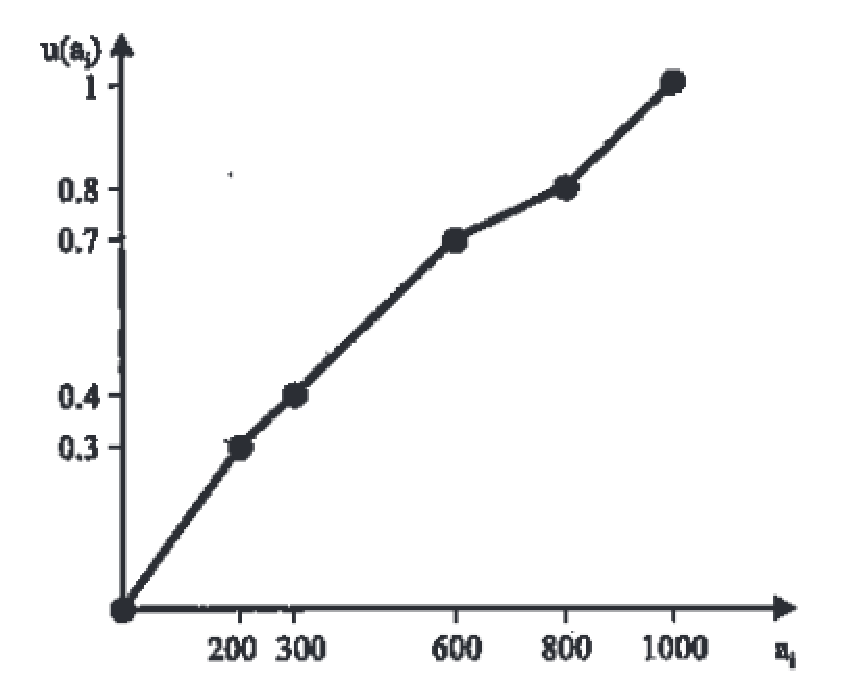
\includegraphics[scale=0.7]{utilmake}
\\
Példa a hasznosságfüggvényre, ami dialógus során keletkezik.
\end{center}

\paragraph{Jelölés: } $a_p = (\alpha: c_1, c_2) \equiv (\alpha \cdot c_1, (1-\alpha) \cdot c_2) $

\paragraph{Feladat: } Legyen $a_p = (0.5:800, 200)$, $a_q = (0.6:600, 300)$ két referencia lottery. Döntsük el, hogy melyiket válasszuk. 

\begin{enumerate}
\item Legyen $c_{min} = 0$ és a $c_{max} = 1000$
\item Az első érték 800, kérdezzük meg a döntéshozót, hogy biztos 800 dolláros nyereség mellett, belevágna-e egy olyan játékba, ahol 20$\%$ eséllyel nyerne 1000 dollárt és 80$\%$  eséllyel semmit. A döntéshozó megmondja, hogy mi a véleménye erről a játékról. Érdemes egy közepes (50$\%$ - 50$\%$ ) eséllyel kezdeni, majd a döntéshozó válasza alapján növelni vagy csökkenteni az esélyt. Ebből megkapható az adott kimenetelhez tartozó hasznossági érték. Legyen például: $800 \sim (0.7:1000, 0)$, $200 \sim (0.1:1000, 0)$, $600 \sim (0.5:1000, 0)$, $300 \sim (0.2:1000, 0)$,
  
\item Összetett lotteryk:  $a_p = (0.5:(0.7:1000, 0), (0.1:1000, 0))$, $a_q = (0.6:(0.5:1000, 0), (0.2:1000, 0))$, a redukciós szabály segítségével hozzuk egyszerűbb alakra: $a_p : (0.5\cdot 0.7+0.5\cdot 0.1) \rightarrow a_p=(0.4:1000, 0)$ , $a_q : (0.6\cdot 0.5+0.4\cdot 0.2) \rightarrow a_q = (0.38:1000, 0)$.
\item $a_p \succ a_q$ mivel $0.4 > 0.38$
\end{enumerate}

Rajzoljuk meg a hasznosságfüggvényt és döntsük el, hogy milyen a döntéshozó kockázati magatartása. (Kockázat kereső)

\paragraph{Az információ ára fejezetnél ismertetett példa hasznosságfüggvény előállítására}

\begin{center}
\begin{tabular}{l|c|c}
\multirow{2}{*}{\bf Cselekvési lehetőségek } &  \multicolumn{2}{c}{ \bf Események }\\
 & $s_1=$ magas infláció (5$\%$) & $s_2=$ alacsony infláció (2$\%$) \\
\hline
  $a_1=$ egy bank részvény & 12 & 9 \\
  $a_2=$ MÁP & 9.995 & 10.295 \\
\end{tabular}
\end{center}
$P(s_1) = 0.55 , P(s_2) = 0.45$ szubjektív valószínűségi értékek (becslések).
A feladat két lotteryje, amiről el kell dönteni, hogy a döntéshozó melyiket válassza az a következő:
$a_p = ( 0.55 \cdot 12 , 0.45 \cdot 9 ) $
$a_q = ( 0.55 \cdot 9.995 , 0.45 \cdot 10.295 ) $

Keressük meg $c_{max}$ és $c_{min}$-t. Legyen $c_{min}$ = 9 , $c_{max}$ = 12. (Megjegyzés, nem feltétlenül a feladatban ismert minimum és maximum a $c_{min}$ és a $c_{max}$, hanem a feladattól függően ettől eltérő is lehetséges. Itt az egyszerűség kedvéért választottuk így.)

Ebből már meg is kaptuk a két bizonyossági egyenértékest: $9 \sim (0: 12,9)$ és $12 \sim (1: 12,9)$.

Vegyük egyesével a maradék két értéket $9.995$ és $10.295$-et biztos eseményként és kérdezzük meg a döntéshozót, hogy emellett a mekkorát kockáztatna a $c_{max}$ eléréséért, ismerve a $c_{min}$ esetleges veszteséget.

Például: Tegyük fel, hogy biztosan nyerünk $9.995$ dollárt. Általában egyesével kérdezzük, hogy játszana-e a biztos esemény helyett ha például: 10$\%$ eséllyel nyerne $c_{max}$-ot vagy, ha 20$\%$ eséllyel nyerne max-ot, ... addig, amíg el nem dönti, hogy mekkora kockázatot vállalna az adott esetben. Például legyen: $9.995 \sim (0.9: 12,9)$ , ekkor csak akkor kockáztatná meg a biztos $9.995$-at, ha 90$\%$-os eséllyel nyerne $c_{max}$-ot. Legyen $10.295 \sim (0.95: 12,9)$ 

$a_p = (0.55:(1: 12,9),(0: 12,9)) = (0.55 \cdot 12, 0.45 \cdot 9)$

$a_q = (0.55:(0.9: 12,9),(0.95: 12,9)) = (0.55 \cdot 0.9 + 0.45 \cdot 0.95) \cdot 12, (0.55 \cdot 0.1 + 0.45 \cdot 0.05) \cdot 9)$

$u(a_p) = 0.55  < u(a_q) = 0.9225$. Tehát a második alternatívát választjuk.

Rajzoljuk meg a hasznosságfüggvényt és döntsük el, hogy milyen a döntéshozó kockázati magatartása. $9.995$ esetén a játék várható pénzértéke $VP(0.9: 12,9)=11.7$, míg $10.295$ esetén $VP(0.95: 12,9)=11.85$. Mivel mindkét várható pénzérték magasabb, mint az érte odaadott biztos nyeremény ezért kockázat kerülő magatartása van a döntéshozónak.

%Most feltesszük, hogy nem tudjuk senkitől sem megtudni a lehetséges valószínűségeket, hanem a döntéshozó segítségével határozzuk meg őket.

%\begin{center}
%\begin{tabular}{l|c|c}
% $A$ & $s_1$ & $s_2$\\
%\hline
%  $a_1$  & $c_1 =  -10 800$ & $c_2 = 2 000$\\
%  $a_2$ & $c_3 = 456$ & $c_4 = 360$ \\
%\end{tabular}
%\end{center}
%A feladat két lotteryje, amiről el kell dönteni, hogy a döntéshozó melyiket válassza az a következő:
%$a_p = (0.25: -10800, 2000)$
%$a_q = (0.25: 456, 360)$

%Keressük meg $c_{max}$ és $c_{min}$-t: $c_{min}$ = $c_1$ , $c_{max}$ = $c_2$. Ebből már meg is kaptuk a két bizonyossági egyenértékest: $c_1 \sim (0: 2000,-10800)$ és $c_2 \sim (1: 2000,-10800)$.

%Vegyük egyesével a maradék $c_3$ és $c_4$-et biztos eseményként és kérdezzük meg a döntéshozót, hogy emellett a mekkorát kockáztatna a $c_{max}$ eléréséért, ismerve a $c_{min}$ esetleges veszteséget.

%Például: Tegyük fel, hogy biztosan nyerünk 456 dollárt. Általában egyesével kérdezzük, hogy játszana-e a biztos esemény helyett ha például: 10$\%$ eséllyel nyerne $c_{max}$-ot vagy, ha 20$\%$ eséllyel nyerne max-ot, ... addig, amíg el nem dönti, hogy mekkora kockázatot vállalna az adott esetben. Például legyen: $c_3 \sim (0.9: 2000,-10800)$ , ekkor csak akkor kockáztatná meg a biztos $c_3$-at, ha 90$\%$-os eséllyel nyerne $c_{max}$-ot. Legyen $c_4 \sim (0.8: 2000,-10800)$ 

%$a_p = (0.25:(0: 2000,-10800),(1: 2000,-10800)) = (0.25 \cdot 0 + 0.75 \cdot 1 : 2000,-10800)$

%$a_q = (0.25:(0.9: 2000,-10800),(0.8: 2000,-10800)) = (0.25 \cdot 0.9 + 0.75 \cdot 0.8 : 2000,-10800)$

%$U(a_p) = 0,75  < U(a_q) = 0,825$. Tehát a második alternatívát választjuk.

%Rajzoljuk meg a hasznosságfüggvényt és döntsük el, hogy milyen a döntéshozó kockázati magatartása. $c_3$ esetén a játék várhatpénzértéke $VP=720$, míg $c_4$ esetén $VP=-560$. Tehát kevert stratégiát alkalmaz.


\subsection{Kockázati magatartás}

\paragraph{Jelölés: } $CE(a_p)$ az $a_p$ lotteryhez tartozó készpénz egyenértékes. 

\begin{center}

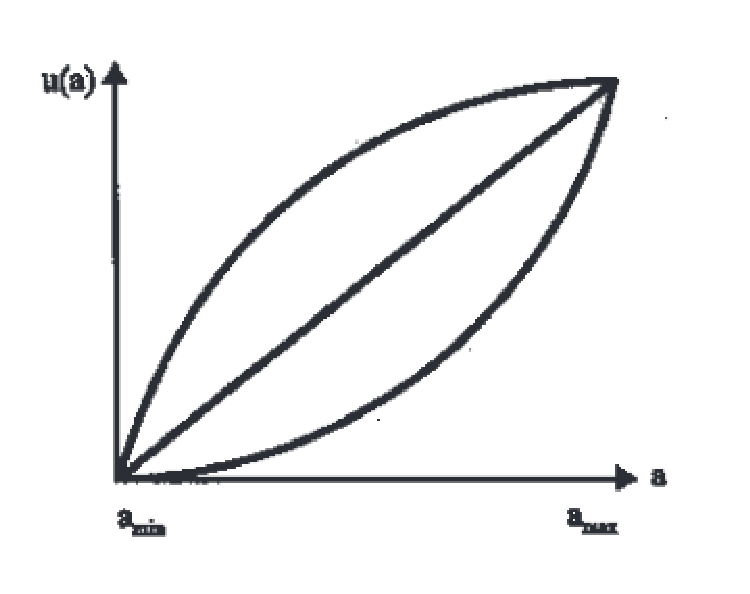
\includegraphics[scale=0.7]{kockazat}
\\
\end{center}

\begin{itemize}
\item $g:$ semleges kockázati magatartás. A döntéshozó ugyanúgy viselkedik sztochasztikus esetben, mint determinisztikus esetben: várható pénzérték alapján dönt. $CE(a_p) = VP(a_p)$
\item $h:$ kockázat kerülő magatartás. A hasznossági függvénye konkáv, bizonyossági egyenértéke szigorúan a várható pénzértéké alatt található: $CE(a_p) < VP(a_p)$
\item $f:$ kockázat kereső magatartás. A hasznossági függvénye konvex, bizonyossági egyenértéke szigorúan a várható pénzértéké felett található: $CE(a_p) > VP(a_p)$
\item lehetnek kevert stratégiák is.
\end{itemize}

\subsection{Többtényezős hasznosság függvény létezése és előállítása}

Többtényezős hasznosság függvény az értékelő függvényhez hasonlóan a dekompozíciós alakok vizsgálatát jelenti. Feltehetjük, hogy tényezőnként ismerjük az egydimenziós hasznosság függvényeket (pl: bizonyossági egyenértékes módszer alapján), így már csak a skálázási konstansok beállítása és a megfelelő függvényalak kiválasztása a feladatunk. Az alak létezésének a vizsgálatához itt is függetlenségi tesztekre lesz szükségünk.

\subsubsection{Függetlenségi tesztek}

Jelölés: $A^p$ kockázatos kimenetelek halmaza:  $a_p=\{c, \alpha\} \in A^p  $ vagy $a_{p} = \{x_i, \alpha_i, x_i \in X_i\}$

\paragraph{Értékfüggetlenség}

Legyen $T=(X_1,...,X_m)$ tényezőhalmaz. $T$ tényezőrészhalmazai \textit{érték-függetlenek} $\Leftrightarrow$ ha $\forall a_p, a_q \in A^p$ (amelyek együttes eloszlásai rendre $\alpha,\beta$): 
\begin{equation}
 a_p \sim a_q \Leftrightarrow \forall i=1..m: \alpha_i=\beta_i
\end{equation}

Ez nehezen teljesülő feltétel, de az additív alak létezésének a feltétele.

\paragraph{Hasznosságfüggetlenség}

Legyen $T=(X_1,...,X_m)$ tényezőhalmaz, $C \subseteq T$ tényezőrészhalmaz,  $C^* \subseteq T $ komplementerhalmaz. Ekkor $C$ hasznosság független $C^*$-tól $\Leftrightarrow$ ha $\forall a_{p}, a_q \in A^p_C:$  egy tetszőleges $x_{C^{*}}^0 \in X_{C^*}$  esetén teljesül minden más $ x_{C^{*}} \in X_{C^*}$ -re, hogy:
%($X_C \in C$, $X_{C^*} \in C^*$)
\begin{equation}
(a_p, x_{C^{*}}^0) \succeq (a_q, x_{C^{*}}^0) 
\Rightarrow
(a_p, x_{C^{*}}) \succeq (a_q, x_{C^{*}}) 
\end{equation}

Hasonló a preferenciafüggetlenséghez, itt lotteryk közötti függőségeket vizsgáljuk.

\paragraph{Preferenciafüggetlenség}

Legyen $T=(X_1,...,X_m)$ tényezőhalmaz, $C \subseteq T$ tényezőrészhalmaz,  $C^* \subseteq T $ komplementerhalmaz. Ekkor $C$ preferencia független $C^*$-tól $\Leftrightarrow$ ha $\forall x_C^{\prime}, x_C^{\prime\prime} \in X_C:$  egy tetszőleges $x_{C^{*}}^0 \in X_{C^*}$  esetén teljesül minden más $ x_{C^{*}} \in X_{C^*}$ -re, hogy:
%($X_C \in C$, $X_{C^*} \in C^*$)
\begin{equation}
(x_C^{\prime}, x_{C^{*}}^0) \succeq (x_C^{\prime\prime}, x_{C^{*}}^0) 
\Rightarrow
(x_C^{\prime}, x_{C^{*}}) \succeq (x_C^{\prime\prime}, x_{C^{*}}) 
\end{equation}
Determinisztikus esethez teljesen hasonlóan.

\textbf{Értékfüggetlenség $\Rightarrow$ Hasznosságfüggetlenség $\Rightarrow$ Preferenciafüggetlenség.}

Értékfüggetlenség $\Rightarrow$ additív forma

Kölcsönös hasznosságfüggetlenség  $\Rightarrow$ multiplikatív forma

Minden tényező ($\{X_i\} = C$) legyen hasznosságfüggetlen a komplementeréhez képest $\Rightarrow$ kvázi additív forma

Minden más esetben  $\Rightarrow$ egyéb formák

\subsection{Additív és multiplikatív hasznosságfüggvény}
\paragraph{A közös alak: kvázi additív hasznosságfüggvény (kifejezhető belőle az additív és a multiplikatív hasznosságfüggvény)}
\begin{equation}
\begin{split}
u(c) = & \sum_{i=1}^n k_i\cdot u_i(x_i)+ \\
&\sum_{i=1}^n \sum_{j>i}^n k_{ij}\cdot u_i(x_i)\cdot u_j(x_j) + \\
&\sum_{i=1}^n \sum_{j>i}^n \sum_{l>j}^n k_{ijl}\cdot u_i(x_i)\cdot u_j(x_j)\cdot u_l(x_l) + ... \\ 
&+k_{1..n}\cdot u_1(x_1)\cdot  ... \cdot  u_n(x_n)
\end{split}
\end{equation}
Ha $k_{ij}, k_{ijl}, ...., k_{1..n}$ egyenlő nullával, akkor megkapjuk belőle az \textbf{additív alakot}:
\begin{equation}
u(c) =  \sum_{i=1}^n k_i\cdot u_i(x_i)
\end{equation}
Megkapható a multiplikatív forma, ha $k_{ij} = K\cdot k_i\cdot k_j, k_{ijl} = K^2\cdot k_i\cdot k_j\cdot k_l, ...., k_{1..n} = K^{n-1}\cdot k_1\cdot ...\cdot k_n$:
\begin{equation}
\label{multiq}
\begin{split}
u(c) = & \sum_{i=1}^n k_i\cdot u_i(x_i)+ \\
&K\cdot \sum_{i=1}^n \sum_{j>i}^n k_{i}\cdot u_i(x_i)\cdot k_{j}\cdot u_j(x_j) + \\
&K^2\cdot \sum_{i=1}^n \sum_{j>i}^n \sum_{l>j}^n k_{i}\cdot u_i(x_i)\cdot k_{j}\cdot u_j(x_j)\cdot k_{l}\cdot u_l(x_l) + ... \\ 
&+K^{n-1}\cdot k_{1}\cdot u_1(x_1)\cdot  ... \cdot  k_{n} \cdot  u_n(x_n)
\end{split}
\end{equation}
Szorozzuk meg mindkét oldalt $K$-val, majd adjunk hozzá mindkét oldalhoz $1$-et:
\begin{equation}
\begin{split}
1 + K\cdot u(c) = & 1 + K\cdot \sum_{i=1}^n k_i\cdot u_i(x_i)+ \\
&K^2\cdot \sum_{i=1}^n \sum_{j>i}^n k_{i}\cdot u_i(x_i)\cdot k_{j}\cdot u_j(x_j) + \\
&K^3\cdot \sum_{i=1}^n \sum_{j>i}^n \sum_{l>j}^n k_{i}\cdot u_i(x_i)\cdot k_{j}\cdot u_j(x_j)\cdot k_{l}\cdot u_l(x_l) + ... \\ 
&+K^{n}\cdot k_{1}\cdot u_1(x_1)\cdot  ... \cdot  k_{n} \cdot  u_n(x_n)
\end{split}
\end{equation}
Ezután a jobboldal szorzattá alakítható az alábbi módon:
\begin{equation}
\begin{split}
1 + K\cdot u(c) = & [1 + K\cdot k_1\cdot u_1(x_1)] \cdot  [1 + K\cdot k_2\cdot u_2(x_2)] \cdot  ...  \cdot  [1 + K\cdot k_n\cdot u_n(x_n)]\\
\end{split}
\end{equation}
Amiből átrendezéssel már kifejezhető a \textbf{multiplikatív alak}: 
\begin{equation}
\begin{split}
u(c) = & \dfrac{1}{K} \cdot  [ \prod_{i=1}^n ( 1 + K\cdot k_i\cdot u_i(x_i)) - 1 ]\\
\end{split}
\end{equation}

\paragraph{$K$ skálázási konstans meghatározása 2D ($n=2$) esetben:} 

Legyen a kiindulási multiplikatív alak olyan alak, amit az additív konstansainak a módosítása során kaptunk a (\ref{multiq}) pontban
\begin{equation}
\begin{split}
u(c) = & k_1\cdot u_1(x_1) + k_2\cdot u_2(x_2)+ \\
&K\cdot  k_{1}\cdot u_1(x_1)\cdot k_{2}\cdot u_2(x_2) \\
\end{split}
\end{equation}
Fejezzük ki $K$-t a $k_i$-kből, ezért legyen $K = \dfrac{1 - (k_1 + k_2)}{k_1\cdot k_2}$. Ekkor:
\begin{equation}
\begin{split}
u(c) = & k_1\cdot u_1(x_1) + k_2\cdot u_2(x_2)+ \\
&\dfrac{1 - (k_1 + k_2)}{ \cancel{k_1\cdot k_2} } \cdot   \cancel{k_{1}}\cdot u_1(x_1)\cdot  \cancel{k_{2}}\cdot u_2(x_2) \\
= & k_1\cdot u_1(x_1) + k_2\cdot u_2(x_2)+ [1 - (k_1 + k_2)]\cdot u_1(x_1)\cdot u_2(x_2) \\
\end{split}
\end{equation}
Ahol az alábbi 3 eset állhat elő:
\begin{enumerate}
\item eset: $k_1 = 0$ és $k_2 = 0 \Rightarrow u(c) = u_1(x_1) \cdot  u_2(x_2), K \rightarrow \infty$. Konjukció, ÉS operátor. 
\item eset: $k_1 = 1$ és $k_2 = 1 \Rightarrow u(c) = u_1(x_1) + u_2(x_2) - u_1(x_1)\cdot  u_2(x_2), K = -1$. Diszjunkció, VAGY operátor.  
\item eset: $k_1 + k_2 = 1 \Rightarrow u(c) = k_1\cdot u_1(x_1) + k_2\cdot u_2(x_2), K = 0 $. Átlag művelet.
\end{enumerate} 

A $k_i$-k tekinthetőek az adott tényezőhöz tartozó súlyozásként, a $K$ pedig azért felelős többek között, hogy a hasznosság a $[0,1]$ intervallumba skálázódjon. A fentiek alapján a $K$ a $[-1, \infty]$ intervallumról vesz fel értéket. Ez határérték vizsgálatokkal kettőnél több tényezős esetben is belátható.


\subsection{Előállítás}

\begin{enumerate}
\item Többtényezős hasznosságfüggvény létezésének verifikálása. Feltételek teljesülése.
\item Az összetevő egydimenziós értékelő függvények megkonstruálása, bizonyossági egyenértékes módszer alapján
\item Megfelelő alakú függvényforma kiválasztása és abból többtényezős hasznosság konstruálása. Főleg a függetlenségi tesztek alapján történik.
\item Konstansok kiválasztása: Kellő mennyiségű preferencia információ alapján felírunk egy konstansokra vonatkozó független egyenletrendszert, megoldjuk. (Konkrét megvalósítással nem foglalkozunk, hasonló a multiplikatív konstansok beállításához.)
\item Konzisztencia ellenőrzés, elemzés. (Döntéshozóval együtt, kérdezéses módszerrel)
\end{enumerate}

\subsection{A hasznossági elmélet felvetéseinek magatartáselméleti kritikái}

Temesi jegyzet, Daniel Kahneman - Gyors és lassú gondolkodás

%\paragraph{Feladat}
%\begin{center}
%\begin{tabular}{c||c|c|c}
% $A$ & $s_1$ (gyenge) & $s_2$ (megfelelő) & $s_3$ (jó)\\
% \hline
% $a_1$&$c^{(1,1)} = (-400, 16)$  &$c^{(1,2)} = (80, 14)$& $c^{(1,3)} = (200, %12)$\\
% $a_2$&$c^{(2,1)} = (10, 20)$  &$c^{(2,2)} = (20, 18)$ & $c^{(1,3)} = (50, %16)$ \\
% $a_3$&$c^{(3,1)} = (-100, 10)$  &$c^{(3,2)} = (0, 8)$ &  $c^{(1,3)} = (100, %8)$\\
%\end{tabular}
%\end{center}
%$P(s_1) = 0,25, P(s_2) = 0,5, P(s_3) = 0,25  $

%\section{Feladatok}
%\begin{enumerate}
%\item Határozza meg a tökéletes információ várható pénzértékét, ha a
% szubjektív valószínűségek: $P(s_1)=$0.4 , $P(s_2)=$0.6 % eredeti: $P(s_1)=$0.6 , $P(s_2)=$0.4
%\vspace{3cm}
%\begin{center}
%\begin{tabular}{l|c|c}
%\multirow{2}{*}{\bf Események} &  \multicolumn{2}{c}{ \bf Cselekvési lehetőségek }\\
% & $a_1=$részvényvásárlás & $a_1=$pénz a bankban\\
% \hline
% $s_1=$raktár épül & 1200 & 660 \\
%  $s_2=$ nem épül raktár& -120 & 600 \\
%\end{tabular}
%\end{center}
%\end{enumerate}

\end{document}
